\documentclass[12pt,a4paper,twoside]{article}
\usepackage{labor}
\begin{document}

%fill for cover and header creation
\newcommand\laboratorynumber{2}
\title{Abbe-Theorie}
\newcommand\supervisor{Robert Nuster}
\newcommand\groupnumber{42}

\newcommand\participantonelastname{Eisner}
\newcommand\participantonefirstname{Nico}
\newcommand\participantoneid{12214121}
\newcommand\participanttwolastname{Waldl}
\newcommand\participanttwofirstname{Philip}
\newcommand\participanttwoid{12214120}
\author{\participantonelastname \ \& \participanttwolastname}

\newcommand\degreeid{UB 033 678}
\newcommand\semester{23WS}
\date{01.12.2023}

%select correct course title
%\newcommand\coursetitle{Einführung in die \\ physikalischen Messmethoden}
%\newcommand\coursetitle{Laborübungen 1: \\ Mechanik und Wärme}
\newcommand\coursetitle{Laborübungen 2: \\ Elektrizität, Magnetismus, Optik}
%\newcommand\coursetitle{Fortgeschrittenen Praktikum 1: \\ Technische Physik}
%\newcommand\coursetitle{Fortgeschrittenen Praktikum 2: \\ Allgemeine Physik}

%\begin{titlepage}
   \begin{center}
       \begin{figure}[H]
            \begin{minipage}[h]{30mm}
                \centerline{
\includegraphics[height=15mm]{cover_nudes/tugraz.png}}
            \end{minipage}
            \hfill
            \begin{minipage}[h]{30mm}
                \centerline{
\includegraphics[height=15mm]{cover_nudes/nawi_graz.png}}
            \end{minipage}
            \hfill
            \begin{minipage}[h]{30mm}
                \centerline{
\includegraphics[height=15mm]{cover_nudes/uni-graz.png}}
            \end{minipage}
        \end{figure}
        
        \large{\emph{Institut für Experimentalphysik der Technischen Universität Graz \\
        \& Institut für Physik der Universität Graz}} \\
        \vspace{5mm}
        
        {\Huge \textbf{\coursetitle}}
        \vspace{5mm}
        
        {\huge \laboratorynumber: \thetitle}
    \end{center}
    
    \vfill
    
    \begin{table}[H]
        \LARGE
        \centering
        \begin{tabular}{r l}
            Betreuer:       & \supervisor \\
            Gruppennummer:  & \groupnumber \\
            \\
            Name:           & \participantonelastname, \participantonefirstname \\
            Matrikelnummer: & \participantoneid \\
            Name:           & \participanttwolastname, \participanttwofirstname \\
            Matrikelnummer: & \participanttwoid \\
            \\
            Kennzahl:       & \degreeid \\
            Datum:          & \semester \ | \thedate
        \end{tabular}
    \end{table}
    \vspace{4cm}
\end{titlepage}
\clearpage
\setcounter{page}{1}

%\maketitle %short title alternative

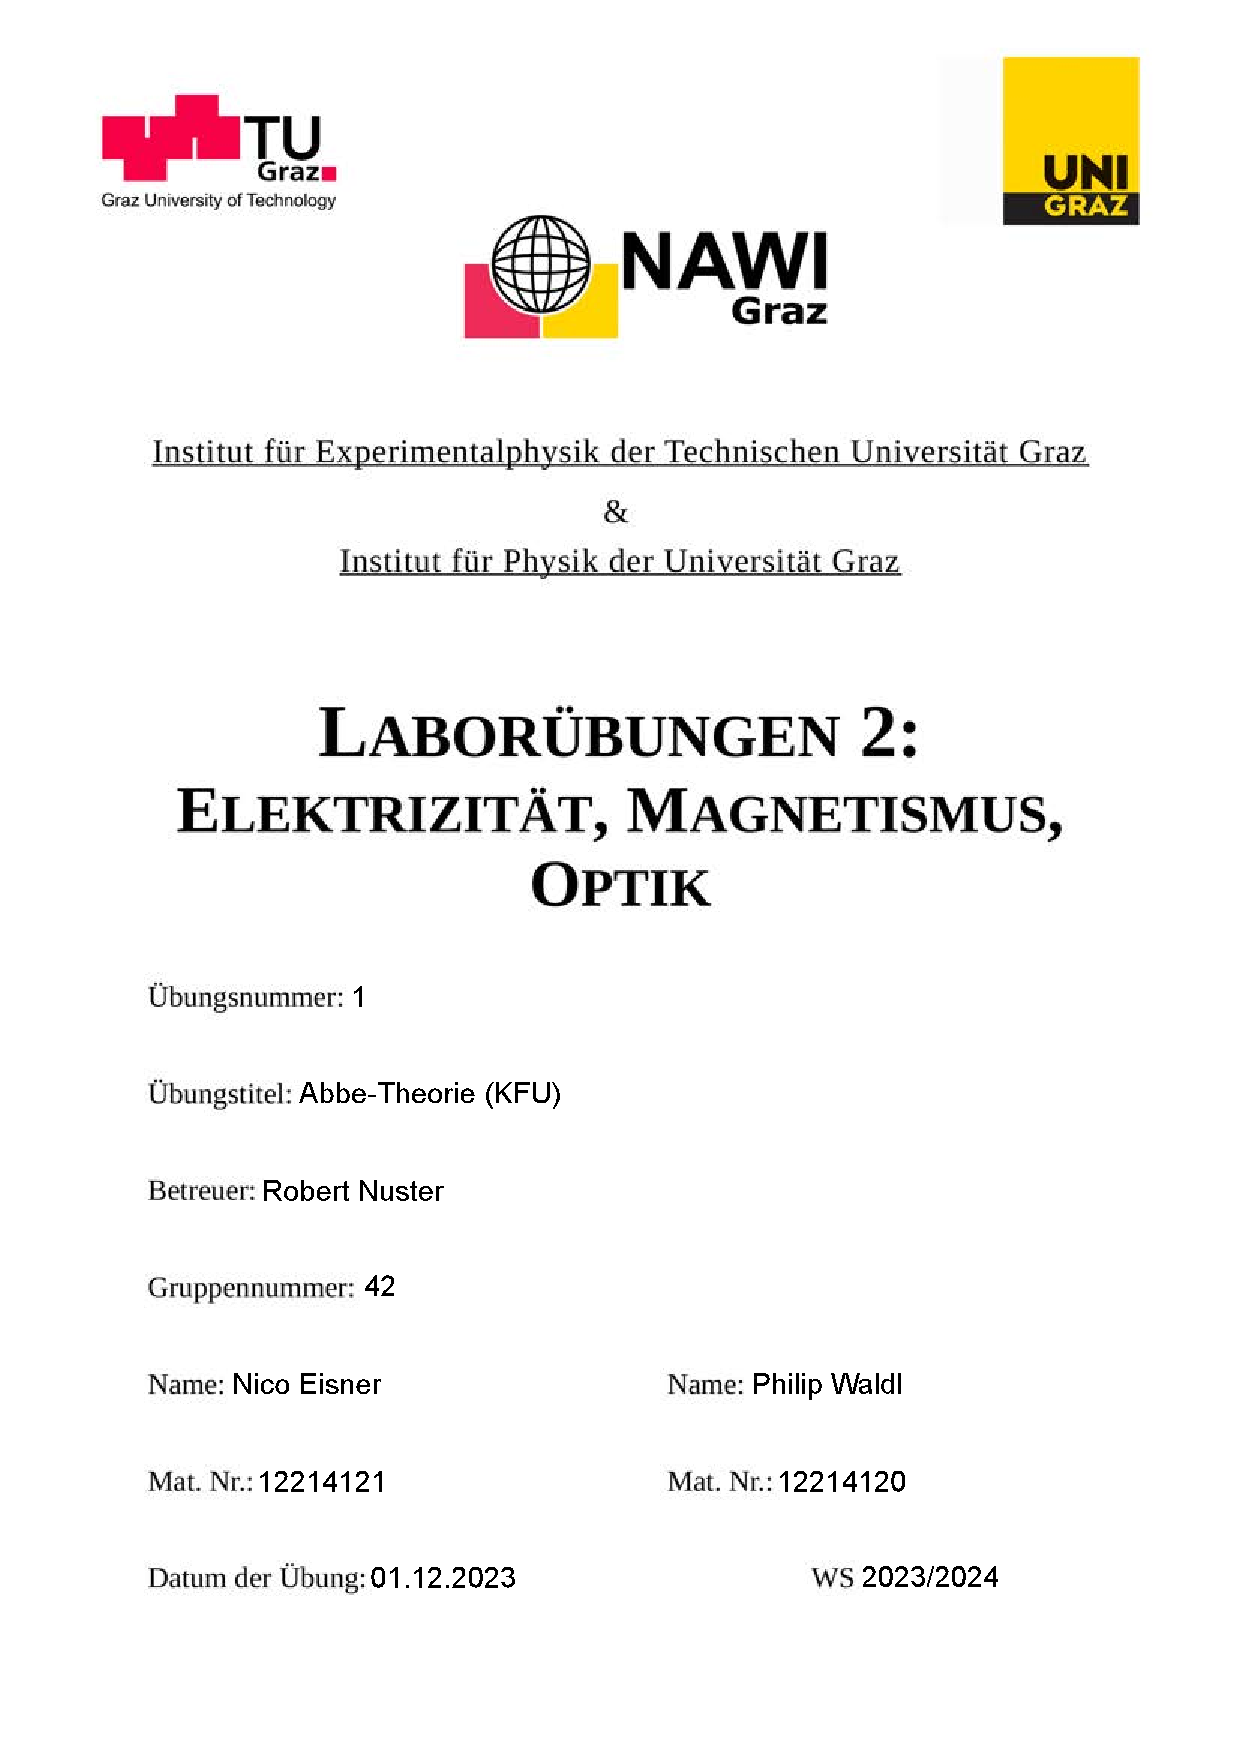
\includepdf[pages={1}]{../Deckblätter/Deckblatt_Abbe.pdf}

\tableofcontents
\newpage

\section{Aufgabenstellung} %jo beschreibn wos gmocht host ------------------------------

Der Versuch Abbe-Theorie behandelt, wie aus dem Namen bereits hervorgeht, die gleichnamige Idee von Ernst Abbe, die in erster Linie die von allen Objekten hervorgehenden Beugungseffekte und deren Zusammenhang mit dem Auflösungsverhalten beinhaltet.
Mittels Experiment der Abbe-Theorie soll dies und einige weitere Eigenschaften dieses Verhaltens nun gezeigt werden.
Die genauen Arbeitsaufträge sehen dabei wie folgt aus:

\begin{itemize}
    \item Vertrautmachen mit dem experimentellen Aufbau
    \item Bestimmung des Auflösungsvermögens einer Linse in Abhängigkeit ihrer numerischen Apertur für
    \begin{itemize}
        \item blaues Licht
        \item rotes Licht
    \end{itemize}
    \item Untersuchung des Zusammenhangs zwischen der Bildauflösung von einem Spaltgitter und der Zahl der transmittierten Beugungsordnungen
    \item  Freies Experimentieren
    \begin{itemize}
        \item Beugungsbild horizontaler Balken
        \item Änderung des Beugungsbild mit dem Abstand der Balken
        \item Grund für Beugungserscheinungen in der Richtung normal zu den Hauptordnungen
        \item Dunkelfeldmikroskopie
        \item Verbindung zu Fourieroptik
    \end{itemize}
\end{itemize}



\section{Voraussetzungen \& Grundlagen} %Grundlagen erklären, Formeln mit erklärung

Das Kapitel Voraussetzungen und Grundlagen wurde basierend auf den literarischen Werken Demtröder \cite{dem2} und dem Script Abbe-Theorie \cite{teachcenter2} verfasst.

\subsection{Auflösungsvermögen und numerische Apertur}

Bei optischen Instrumenten wird das Auflösungsvermögen $\Delta x_{min}$ als der Minimalabstand zwischen zwei Punkte definiert, bei dem das Gerät diese noch als zwei punktförmige Objekte unterscheiden kann.
Dieser Versuch kann mit in dieser Hinsicht mit einem Mikroskop verglichen werden, dessen Auflösungsvermögen wie folgt definiert ist:

\begin{equation}
    \label{eq:Auflösungsvermögen}
    \centerline{$\Delta x_{min} = 0.61\frac{\lambda}{NA}$}
\end{equation}

\noindent
Dabei stellt $\lambda$ die Wellenlänge des verwendeten Lichtes und NA die numerische Apertur des optischen Instrumentes, also grob gesagt dem Öffnungswinkel, durch den das Licht eintreten kann, dar.
Letzteres ist wiederum definiert als:

\begin{equation}
    \label{eq:NA}
    \centerline{$NA = n sin(\alpha)$}
\end{equation}

\noindent
mit n als Brechzahl des Mediums und $\alpha$ dem halben Öffnungswinkel des Lichtkegels. Da n in der Regel (sofern Luft als Medium dient) einen Wert von ziemlich genau 1 annimmt und $\alpha$ als $\tan^{-1}(\frac{R}{g})$ (R ... Linsenradius, g ... Gegenstandsweite) angesehen werden kann (veranschaulicht in Abbildung \ref{fig:NA-Skizze}), lässt sich die Formel für die numerische Apertur auch folgendermaßen umschreiben:

\begin{equation}
    \label{eq:NA-umgeschrieben}
    \centerline{$NA = sin(\tan^{-1}(\frac{R}{g}))$}
\end{equation}

\begin{figure}[H]
    \centering
    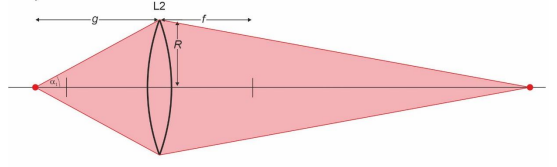
\includegraphics[width=0.5\linewidth]{nudes/NA-Skizze.png}
    \caption{Schematische Darstellung Bestimmmung NA \cite{teachcenter2}}
    \label{fig:NA-Skizze}
\end{figure}


\subsection{Variation der numerischen Apertur}

Der Einfluss des numerischen Apertur kann nur experimentell gezeigt werden, indem man sie variiert. Hierfür bietet es sich an, Linsen mit verschiedenen Durchmessern (Veränderung von R in \ref{eq:NA-umgeschrieben}) zu verwenden, oder der Einsatz einer Lochblende in der hinteren Brennebene der Linse.
Wie genau die numerische Apertur das Auflösungsverhalten beeinflusst wird im folgenden Experiment gezeigt.


\subsection{Abbesche Abbildungstheorie}

Wie im Kapitel Aufgabenstellung bereits einleitend erwähnt, besagt die Abbe Theorie, dass von jedem Objekt Beugungsmaxima hervorgehen und die Auflösung einen Zusammenhang zur Zahl der Beugungsmaxima besitzt.
Wichtig hierbei ist außerdem die Verwendung eines Gitters, dessen Spaltbreite dem halben Spaltabstand entspricht. Somit fehlen fehlen dem Gitter die gradzahligen Beugungsmaxima und am Bild hinter dem Vielfachspalt sind nur die ungradzahligen Maxima erkennbar (wird im Verlauf des Experimentes noch gezeigt).
Mit Hilfe des Tools für die grafische Darstellung solcher Muster von Leifi-Physik \cite{leifi} kann dieses Scenario theoretisch simuliert werden:

\begin{figure}[H]
    \centering
    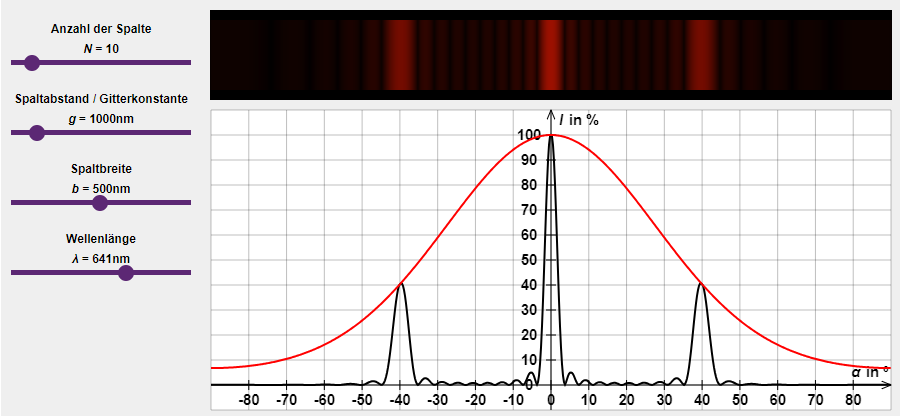
\includegraphics[width=0.4\linewidth]{nudes/VG-Simulation10Nrot.png}
    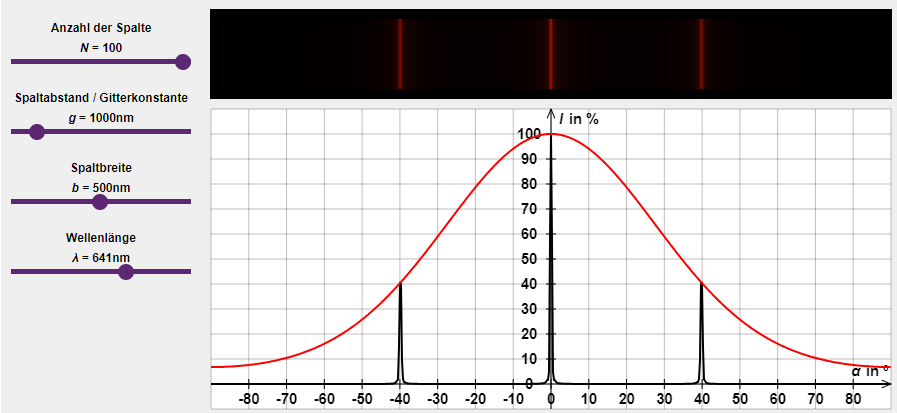
\includegraphics[width=0.4\linewidth]{nudes/VG-Simulation100Nrot.png}
    \caption{Simulation der Maxima einer Gitterbeugung von rotem Licht mit 10/100 Spaltöffnungen}
    \label{fig:SimulationRot}
\end{figure}

\begin{figure}[H]
    \centering
    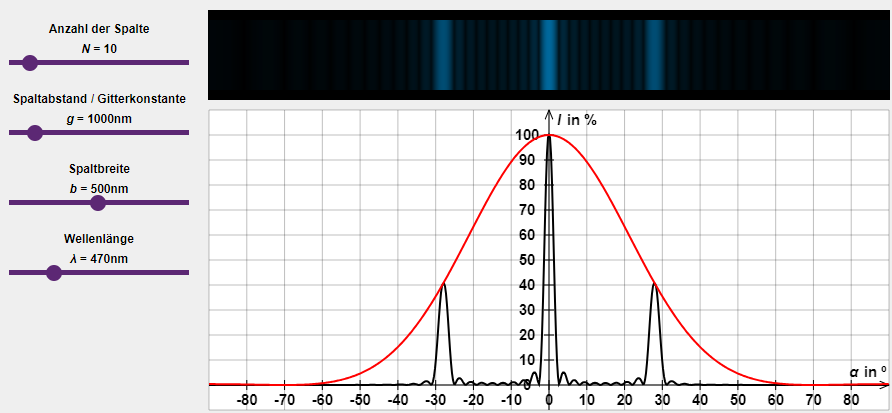
\includegraphics[width=0.4\linewidth]{nudes/VG-Simulation10Nblau.png}
    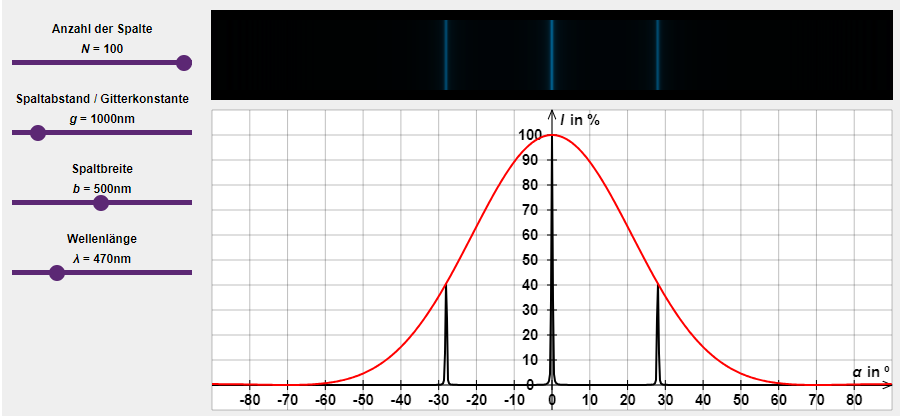
\includegraphics[width=0.4\linewidth]{nudes/VG-Simulation100Nblau.png}
    \caption{Simulation der Maxima einer Gitterbeugung von blauem Licht mit 10/100 Spaltöffnungen}
    \label{fig:SimulationBlau}
\end{figure}


\subsection{Wichtige Zusammenhänge}

Für eine erfolgreiche Auswertung der Daten werden außerdem folgende Zusammenhänge benötigt:

\begin{equation}
    \label{eq:avg}
    \centerline{Mittelwert \\ $M = \frac{1}{n}\sum_{i = 1}^{n} x_{i} $ \\ }
\end{equation}

\begin{equation}
    \label{eq:WZ-NA}
    \centerline{Numerische Apertur \\ $NA = \frac{D_{Blende}}{2f_{2}}$ \\ $\Delta NA = \vert \frac{\partial NA}{\partial D_{Blende}} * \Delta D_{Blende} \vert + \vert \frac{\partial NA}{\partial f_{2}} * \Delta f_{2} \vert $}
\end{equation}

\begin{equation}
    \label{eq:WZ-dTheo}
    \centerline{Auflösungsvermögen theoretisch \\ $d_{th} = 0.61\frac{\lambda}{NA}$ \\ $\Delta d_{th} = \vert \frac{\partial d_{th}}{\partial \lambda} * \Delta \lambda \vert + \vert \frac{\partial d_{th}}{\partial NA} * \Delta NA \vert $}
\end{equation}

\begin{equation}
    \label{eq:WZ-fr}
    \centerline{Räumliche Frequenz \\ $f_{R} = 2^{n_{g}^{\frac{n_{E}-1}{6}}}$ \\ $\Delta f_{R} = \vert \frac{\partial f_{R}}{\partial n_{g}} * \Delta n_{g} \vert + \vert \frac{\partial f_{R}}{\partial n_{E}} * \Delta n_{E} \vert $}
\end{equation}

\begin{equation}
    \label{eq:WZ-dExp}
    \centerline{Auflösungsvermögen experimentell \\ $d_{exp} = \frac{1}{f_{R}}$ \\ $\Delta d_{exp} = \vert \frac{\partial d_{exp}}{\partial f_{R}} * \Delta f_{R} \vert$}
\end{equation}


    

\section{Versuchsanordnung} %mit skizze kurz beschreiben ------------------------------

Der Aufbau des Experimentes ist im Grunde sehr simpel. Es besteht aus einer Aluschiene, auf der acht verschiedene Module in einem bestimmten Abstand angebracht sind. 

\begin{figure}[H]
    \centering
    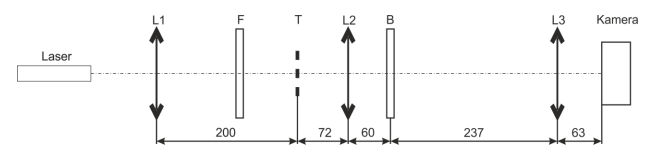
\includegraphics[width=0.8\linewidth]{nudes/VersuchsaufbauTheoretisch.png}
    \caption{Optischer Aufbau des Experiments; L1: f1 = 200mm, F: Filterrad mit roter/blauer LED, Graufilter und freiem
    Durchgang, T: Testobjekt; L2: f2 = 60mm; B: Filterrad mit 2/3/6 mm Lochblenden, einer Irisblende und einer
    Drahtblende, L3(einklappbar): f3 = 50mm. \cite{teachcenter2}}
    \label{fig:VersuchsaufbauTheoretisch}
\end{figure}

\begin{figure}[H]
    \centering
    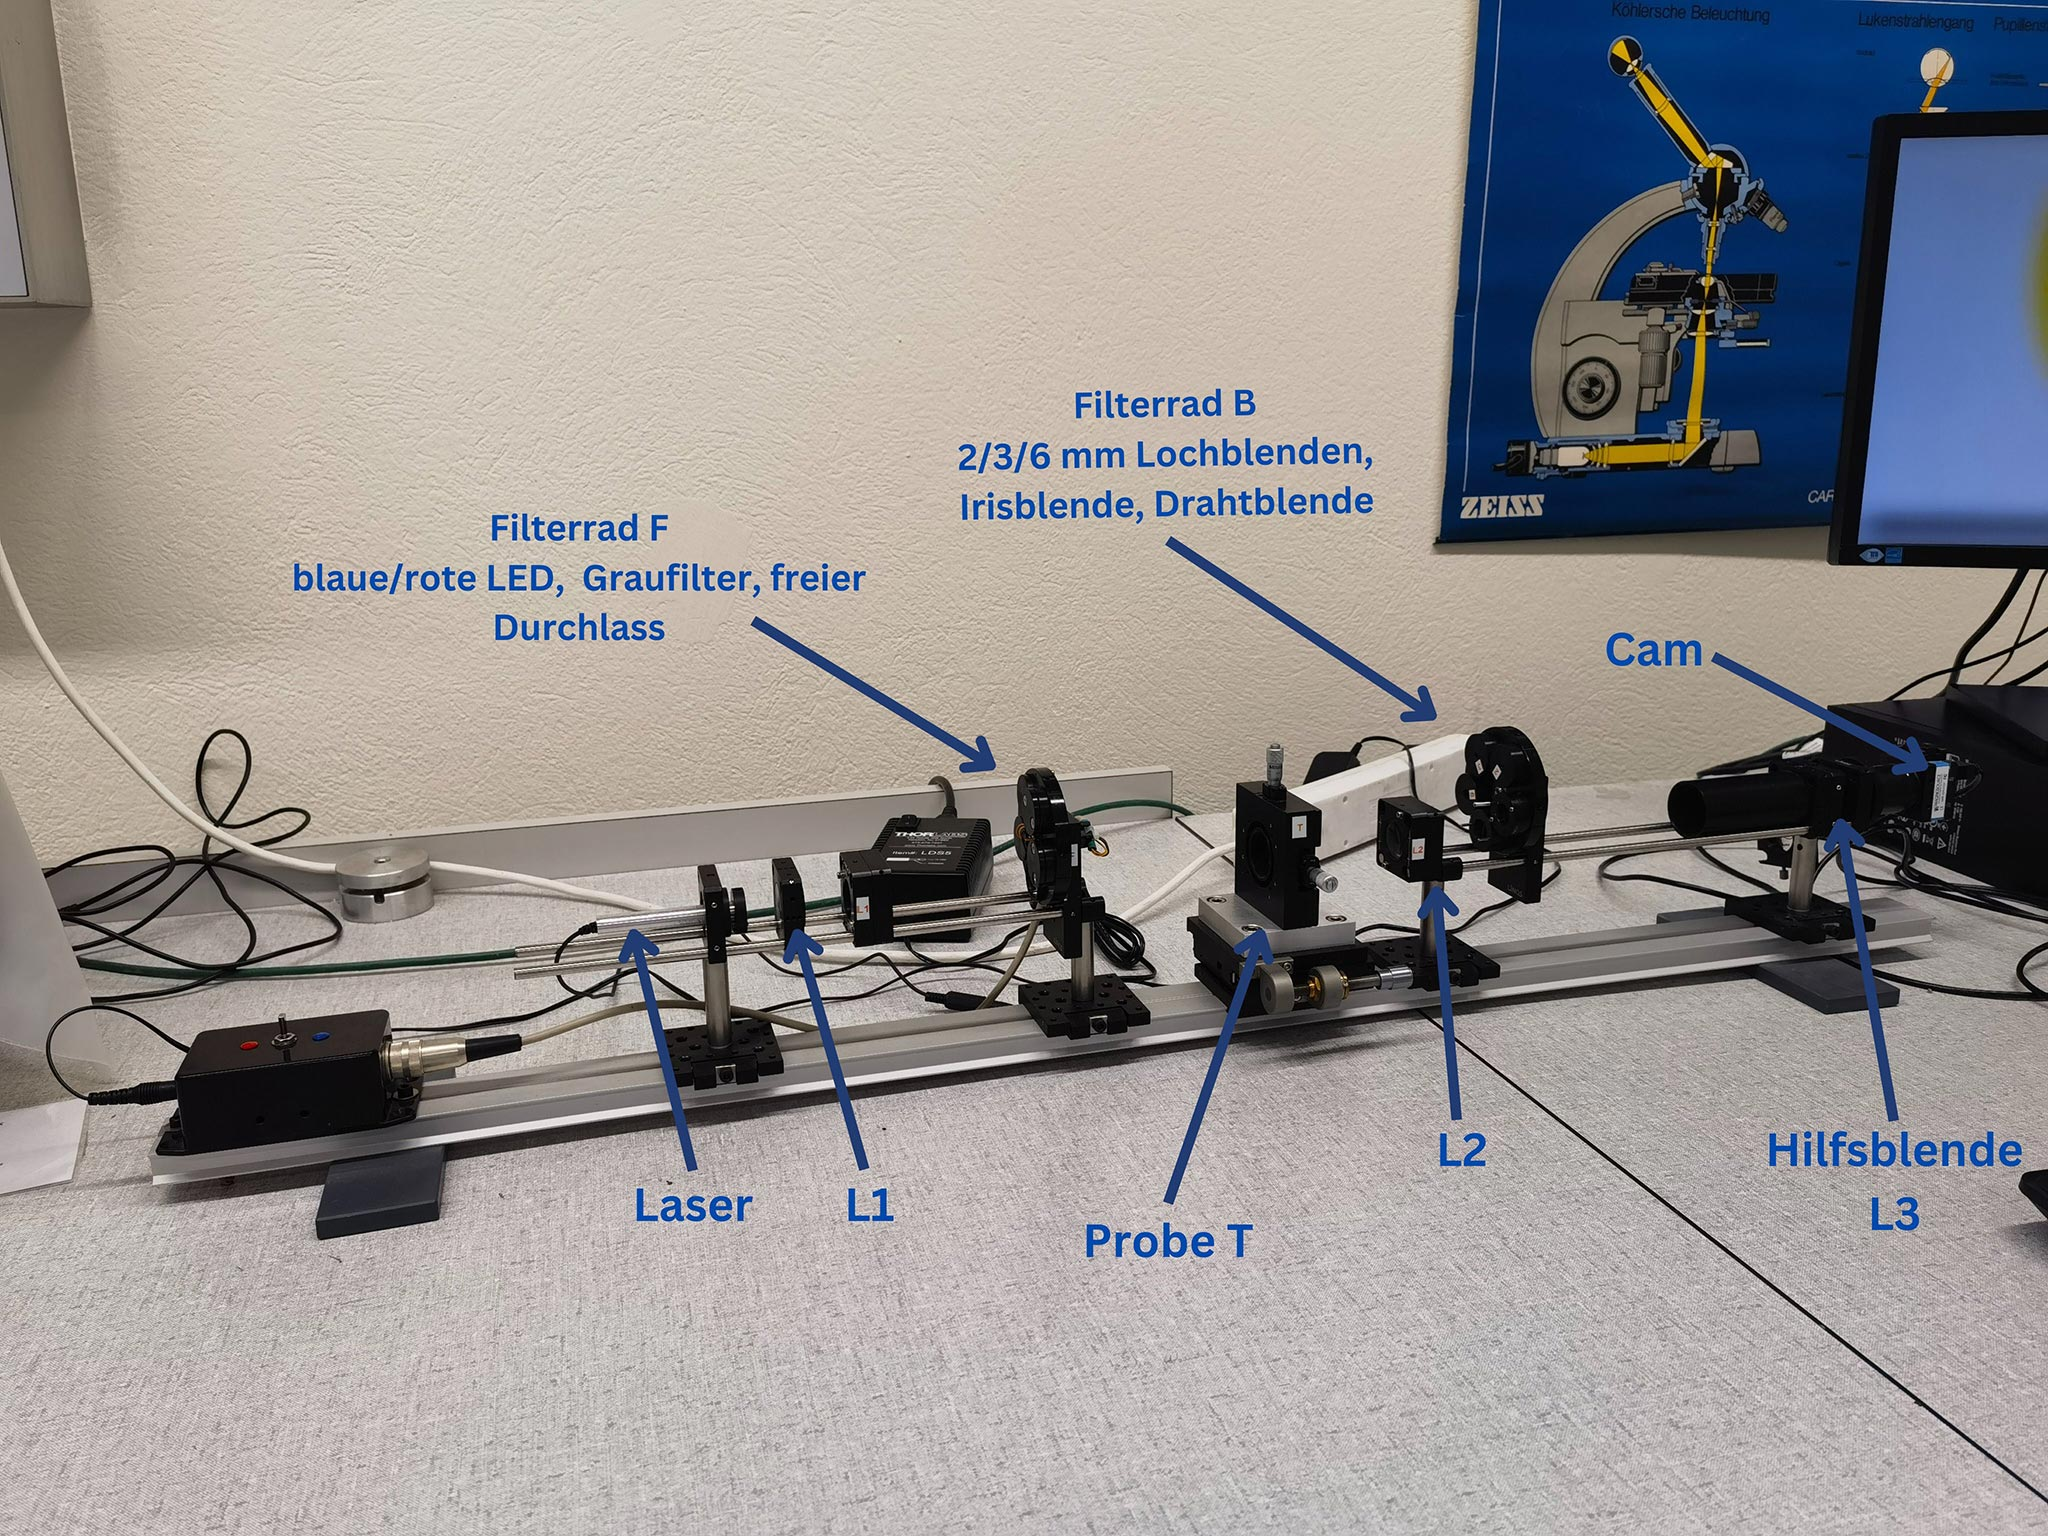
\includegraphics[width=0.7\linewidth]{nudes/VersuchsaufbauIRLbeschriftet.jpg}
    \caption{Versuchsaufbau laut Abbildung \ref{fig:VersuchsaufbauTheoretisch}}
    \label{fig:Versuchsaufbau}
\end{figure}

Die Einzelteile mit Beschreibung sind in folgender Tabelle ersichtlich:

\begin{table}[H]
    \centering
    \caption{Aufbau: Module}
    \label{tab:Aufbau}
    \begin{tabular}{| l | l | l | l |}
        \hline
        Nr.  & Modul & Bezeichnung  & Eigenschaft \\
        \hline
        1 & Laser & Laser & λ= 531,9 nm \\
        2 & Sammellinse 1 & L1 & f1 = 200 mm \\
        3 & Filterrad & F & rote/blauer LED, Graufilter und freier Durchgang \\
        4 & Testobjekt bzw. Probe & T &  \\
        5 & Sammellinse 2 & L2 & f2 = 60 mm \\
        6 & Filterrad & B & 2/3/6 mm Lochblenden, Irisblende und Drahtblende \\
        7 & Sammellinse 3 & L3 & f3 =  50 mm \\
        8 & Kamera & Kamera & Fotosensor mit PC/IC Capture Verbindung \\
        \hline
    \end{tabular}
\end{table}

\noindent
Mit dem Drehrad an der Seite des Testobjektes ist es außerdem möglich, die Schärfe der Probe zu adjustieren. \newline

\noindent
Teil der Vorbereitung war es auch, mögliche Strahlengänge durch diesen Aufbau theoretisch zu zeichnen. Diese sind in nachfolgenden Abbildungen zu sehen.

\begin{figure}[H]
    \centering
    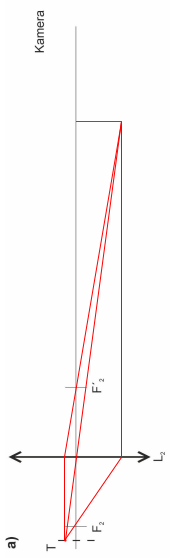
\includegraphics[width=0.3\linewidth, angle=-90]{nudes/Strahlenganga.png}
    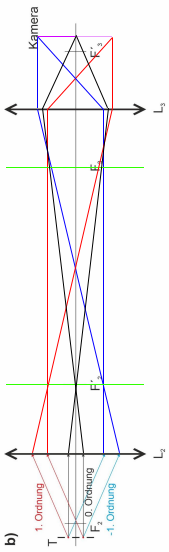
\includegraphics[width=0.3\linewidth, angle=-90]{nudes/Strahlengangb.png}
    \caption{Theoretische Strahlengänge}
    \label{fig:theorStrahlengang}
\end{figure}

\section{Geräteliste} %jo holt a listn ------------------------------

    \begin{table}[H]
        \centering
        \caption{Im Versuch verwendete Geräte und Utensilien.}
        \label{tab:geraete}
        \begin{tabular}{| l | l | l | l | l |}
            \hline
            Gerät   & Bezeichnung  & Hersteller  & Eigenschaften  & Unsicherheit \\
            \hline
            Sammellinse & L1 & {n.a} & f1 = 200 mm & 1 mm \\
            Sammellinse & L2 & {n.a} & f1 = 60 mm  & 1 mm \\
            Sammellinse & L3 & {n.a} & f1 = 50 mm  & 1 mm \\
            Laser & Laser & Thorlabs & λ= 531,9 nm & {n.a.} \\
            LED blau & LEDb & Cxxx & λ= 470 nm & 5 nm \\
            LED rot & LEDr & Cxxx & λ= 635 nm & 5 nm \\
            Kamera & Kamera & The Imaging Source & {n.a.} & {n.a.}\\
            Kamera & {n.a.} & The Imaging Source & {n.a.} & {n.a.}\\
            SciDAVis & {n.a.} & Cxxx & {n.a.} & {n.a.} \\
            \hline
        \end{tabular}
    \end{table}


\section{Versuchsdurchführung \& Messergebnisse} %nachvollziehbar und klar dargestellt ------------------------------

Bevor die eigentlichen Messvorgänge starten konnten, war es laut Aufgabe 0 wichtig, sich zuvor mit dem Aufbau und Messinstrumenten vertraut zu machen. 
Der erste Blick fällt dabei auf das Testobjekt des Versuches, dargestellt in folgender Abbildung \ref{fig:Testelement}.

\begin{figure}[H]
    \centering
    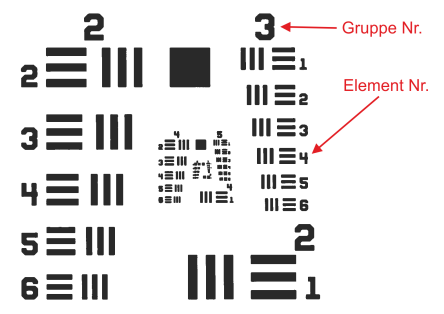
\includegraphics[width=0.6\linewidth]{nudes/Testelement.png}
    \caption{Testelement des Versuches \cite{teachcenter2}}
    \label{fig:Testelement}
\end{figure}

\noindent
Wie sich erkennen lässt, besteht dieses aus mehreren Strichblöcken, die sich aus drei gleichweit voneinander entfernten Linien (je drei horzizontal und drei vertikal ausgerichtet) zusammensetzen.
Zur genauen Beschriftung wurden die Blöcke in Gruppen eingeteilt, welche sich jeweils auf einer Seite der Spirale befinden und durch die großen Zahlen gelabelt sind. Jede Gruppe besteht weiters aus sechs dieser horizontalen- und vertikalen Strichelemente, gekennzeichnet mit einer weiteren Nummerierung.
Mit der nachfolgenden Tabelle \ref{tab:fR-Tabelle} ist jedem Element der Gruppen ein eindeutiger Wert für die räumliche Frequenz $f_{R}$ in 1/mm zugeteilt.

\begin{table}[H]
    \centering
    \caption{Räumliche Frequenz der Balken in 1/mm für die unterschiedlichen Elemente des Testobjektes \cite{teachcenter2}}
    \label{tab:fR-Tabelle}
    \begin{tabular}{|l|llllllllll|}
    \hline
    Element Nr. & \multicolumn{10}{l|}{Gruppen Nr.}                                                                                                                                                                                                                                      \\ \hline
                & \multicolumn{1}{l|}{-2}    & \multicolumn{1}{l|}{-1}    & \multicolumn{1}{l|}{0}    & \multicolumn{1}{l|}{1}    & \multicolumn{1}{l|}{2}    & \multicolumn{1}{l|}{3}     & \multicolumn{1}{l|}{4}     & \multicolumn{1}{l|}{5}    & \multicolumn{1}{l|}{6}     & 7     \\ \hline
    1           & \multicolumn{1}{l|}{0,250} & \multicolumn{1}{l|}{0,500} & \multicolumn{1}{l|}{1,00} & \multicolumn{1}{l|}{2,00} & \multicolumn{1}{l|}{4,00} & \multicolumn{1}{l|}{8,00}  & \multicolumn{1}{l|}{16,00} & \multicolumn{1}{l|}{32,0} & \multicolumn{1}{l|}{64,0}  & 128,0 \\ \hline
    2           & \multicolumn{1}{l|}{0,280} & \multicolumn{1}{l|}{0,561} & \multicolumn{1}{l|}{1,12} & \multicolumn{1}{l|}{2,24} & \multicolumn{1}{l|}{4,49} & \multicolumn{1}{l|}{8,98}  & \multicolumn{1}{l|}{17,95} & \multicolumn{1}{l|}{36,0} & \multicolumn{1}{l|}{71,8}  & 144,0 \\ \hline
    3           & \multicolumn{1}{l|}{0,315} & \multicolumn{1}{l|}{0,630} & \multicolumn{1}{l|}{1,26} & \multicolumn{1}{l|}{2,52} & \multicolumn{1}{l|}{5,04} & \multicolumn{1}{l|}{10,10} & \multicolumn{1}{l|}{20,16} & \multicolumn{1}{l|}{40,3} & \multicolumn{1}{l|}{80,6}  & 161,0 \\ \hline
    4           & \multicolumn{1}{l|}{0,353} & \multicolumn{1}{l|}{0,707} & \multicolumn{1}{l|}{1,41} & \multicolumn{1}{l|}{2,83} & \multicolumn{1}{l|}{5,66} & \multicolumn{1}{l|}{11,30} & \multicolumn{1}{l|}{22,62} & \multicolumn{1}{l|}{45,3} & \multicolumn{1}{l|}{90,5}  & 181,0 \\ \hline
    5           & \multicolumn{1}{l|}{0,397} & \multicolumn{1}{l|}{0,793} & \multicolumn{1}{l|}{1,59} & \multicolumn{1}{l|}{3,17} & \multicolumn{1}{l|}{6,35} & \multicolumn{1}{l|}{12,70} & \multicolumn{1}{l|}{25,39} & \multicolumn{1}{l|}{50,8} & \multicolumn{1}{l|}{102,0} & 203,0 \\ \hline
    6           & \multicolumn{1}{l|}{0,445} & \multicolumn{1}{l|}{0,891} & \multicolumn{1}{l|}{1,78} & \multicolumn{1}{l|}{3,56} & \multicolumn{1}{l|}{7,13} & \multicolumn{1}{l|}{14,30} & \multicolumn{1}{l|}{28,50} & \multicolumn{1}{l|}{57,0} & \multicolumn{1}{l|}{114,0} & 228,0 \\ \hline
\end{tabular}
\end{table}

\noindent
Das Testobjekt wird für spätere Messwerte benötigt. Weiters wurde der Pc gestartet und das Programm IC-Capture gestartet. Nachdem die Kamera verbunden wurde, wurden einige Einstellungen getroffen:

\begin{itemize}
    \item Bildformat: "RGB1280-720" - 3
    \item Histogramm eingeblendet - 2
\end{itemize}

\begin{figure}[H]
    \centering
    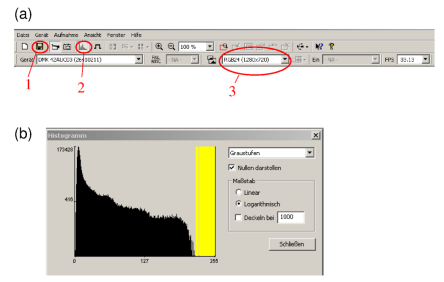
\includegraphics[width=0.5\linewidth]{nudes/IcCaptureSettings.png}
    \caption{a.) IcCapture Einstellungen b.) eingeblendetes Histogramm}
    \label{fig:IcCaptureSettings}
\end{figure}

\noindent
Das Histogramm dient dazu, die Belichtung des aufzunehmenden Bildes zu adjustieren. Hierfür sollte die ''Exposure-Time'' so eingestellt werden, dass der gelbe Balken rechts gerade noch zu sehen ist, um das Bild optimal zu belichten.


\subsection{Vertrautmachen mit dem Versuch}

Um nun zu Aufgabe 0 zurückzukommen, zu Beginn wurde eine der beiden LEDs (rot oder blau) eingeschaltet und ungehindert durch die Vorrichtung gelassen. Dann wurde die Hilfslinse L3 weggeklappt und die verstellbare Irisblende auf Filterrad B in den Strahlengang gedreht. 
Mit dem kleinen Hebel kann diese geöffnet bzw. geschlossen werden, wobei zunächst für ersteres gesorgt wurde. Am Verschiebeschlitten des Testobkjektes konnte nun auf das Testobjekt fokusiert und dieses somit scharf gestellt werden. 
Mit den Mikrometerschrauben am Verschiebeschlitten des Testelementes konnte nun unterschiedliche Bereiche davon dargestellt werden, wobei die obere Schraube eine Änderung an der x-Achse und die seitliche Schraube eine Änderung auf der y-Achse bewirkt. 
Nun soll ein Bild des Testelementes mit geöffneter- und beinahe geschlossener Irisblende aufgenommen werden. Das Messergebnisse ist in nachfolgenden Abbildungen zu erkennen.

\begin{figure}[H]
    \centering
    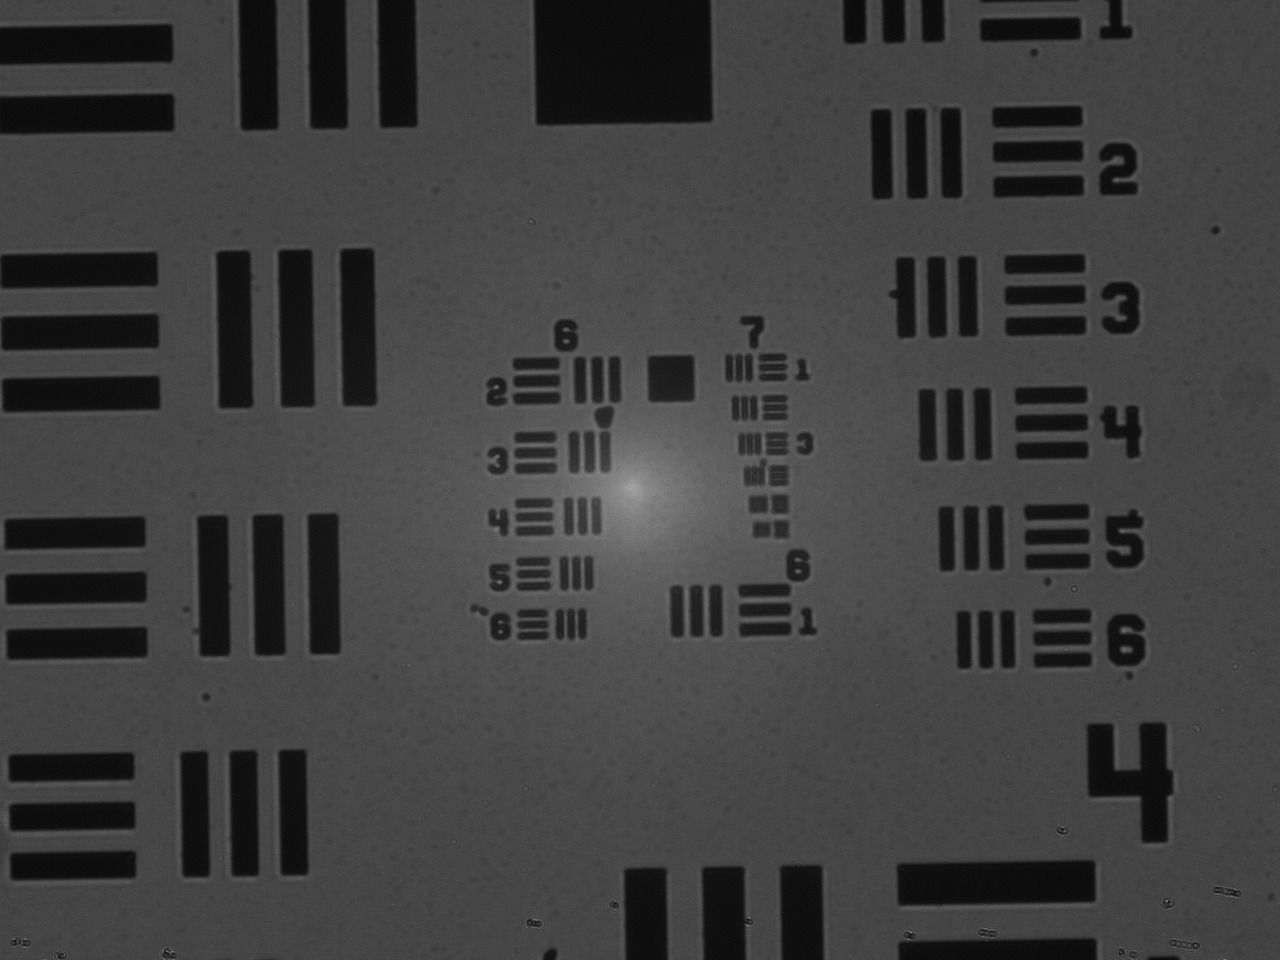
\includegraphics[width=0.4\linewidth]{nudes/AbbeTheorie/Aufgabe 0/scharf-blende-offen.jpg}
    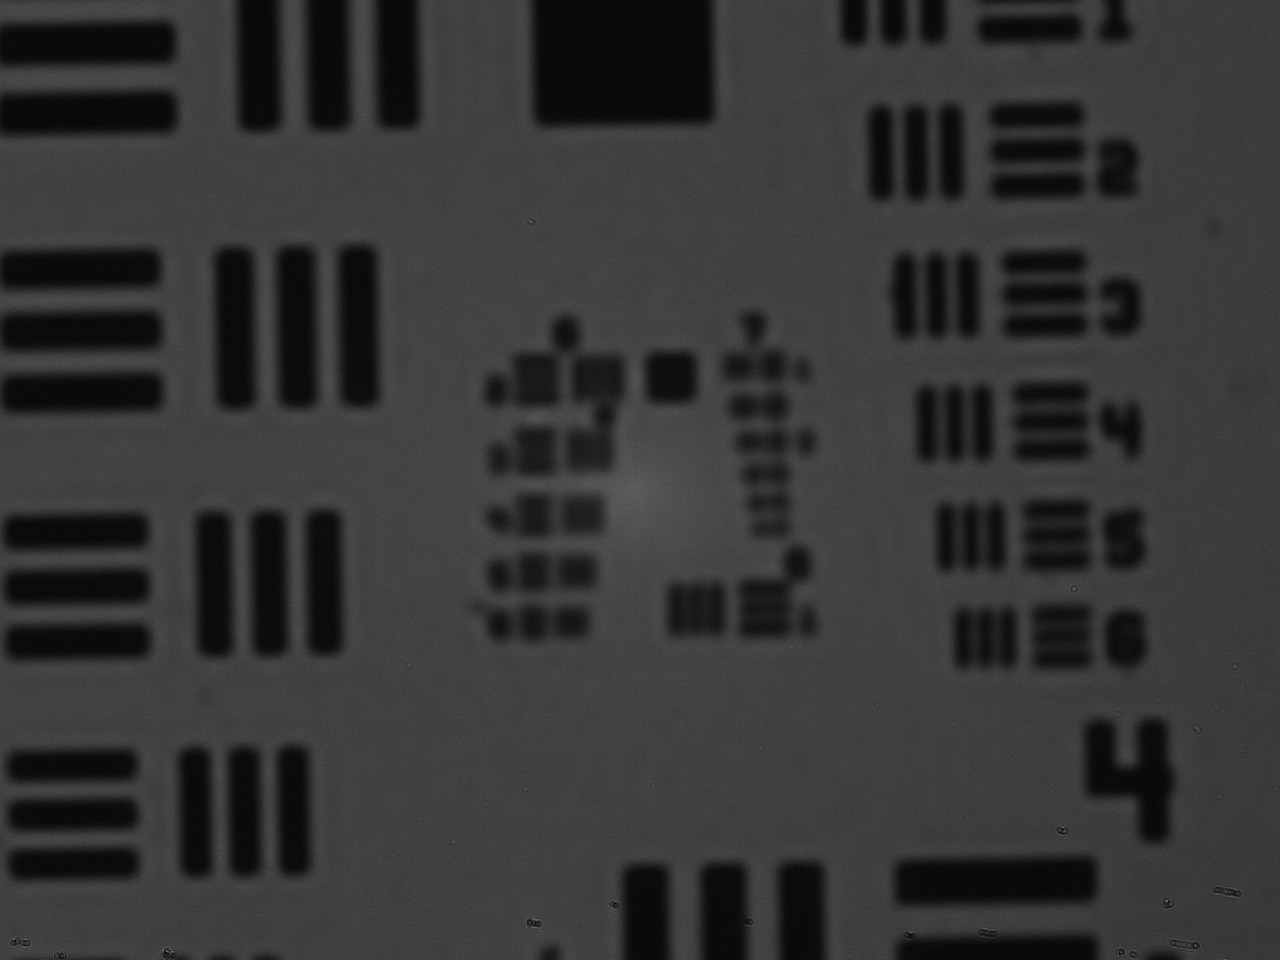
\includegraphics[width=0.4\linewidth]{nudes/AbbeTheorie/Aufgabe 0/scharfgestellt-blende-zu.jpg}
    \caption{Testelement mit geöffneter/fast geschlossener Irisblende}
    \label{fig:Aufgabe0}
\end{figure}


\subsection{Quantitative Bestimmung des Auflösungsvermögens}

Beim nächsten Punkt drehte sich alles um das Auflösungsvermögen. Dieses galt es nämlich in Abhängigkeit der numerischen Apertur für zwei verschiedene Wellenlängen (rotes/blaues Licht) zu bestimmen. 
Hierfür wurde die benötigte LED eingeschaltet und in den Strahlengang eingebracht. Mit Hilfe der drei verschiedenen Lochblenden am Filterrad B kann die numerische Apertur gemäß Formel \ref{eq:NA-umgeschrieben} (Änderung des Radius R) variiert werden. \newline

\noindent
Zu beachten gibt es einen Abbildungsfehler, der durch die LED-Linse entsteht und einen weißen Punkt am Bild erscheinen lässt. Durch verschieben des Testelement mittels der beiden Drehschrauben soll dieser Punkt an einen für die Messung unwichtigen Ort (am Besten die Mitte der Spirale) verschoben werden. \newline

\noindent
Nun sollen die Bilder für jede Lochblende untersucht werden. Dabei wird jenes Balkenelement (horizontal und vertikal) bestimmt, welches nichtmehr erkennbar ist. Dieses Element gilt es in der Tabelle \ref{tab:fR-Tabelle} ausfindig zu machen und die daraus folgenden Werte zu notieren.
Bei dieser Herangehensweiße gibt es einen Ermessensspielraum bei der Entscheidung, ob die Balken noch erkennbar sind oder nicht. Dieser Spielraum stellt für die spätere Auswertung die Unsicherheit dar.

\begin{table}[H]
    \centering
    \caption{Messung des Auflösungsvermögens für rotes Licht}
    \label{tab:MessungenAuflösungsvermögenRot}
    \begin{tabular}{| l | l | l | l | l | l |}
        \hline
        Nr. & Blende / mm & Gruppe & Element & \multicolumn{2}{|c|}{Unsicherheit} \\
        \hline
        1 & 2 & 5 & 4 & 5/3 & 5/5 \\
        2 & 3 & 6 & 1 & 5/6 & 6/2 \\
        3 & 6 & 6 & 5 & 6/4 & 6/6 \\
        \hline
    \end{tabular}
\end{table}

\begin{table}[H]
    \centering
    \caption{Messung des Auflösungsvermögens für blaues Licht}
    \label{tab:MessungenAuflösungsvermögenBlau}
    \begin{tabular}{| l | l | l | l | l | l |}
        \hline
        Nr. & Blende / mm & Gruppe & Element & \multicolumn{2}{|c|}{Unsicherheit} \\
        \hline
        1 & 2 & 5 & 5 & 5/4 & 5/6 \\
        2 & 3 & 6 & 3 & 6/2 & 6/4 \\
        3 & 6 & 7 & 1 & 6/6 & 7/2 \\
        \hline
    \end{tabular}
\end{table}




\subsection{Zusammenhang Auflösung Spaltgitterbildes und Anzahl Beugungsordnungen}

Im weiteren Versuchsverlauf soll nun der Zusammenhang zwischen Bildauflösung und Beugungsordnungen dargestellt werden. 
Hierfür wird zunächst das Testobjekt mit der roten LED und dem Hebel an der Testelementschiene fokusiert. Dann sollen die drei horizontale Balken des Elementes 3/4 ausfindig gemacht werden.
Sobald dies erreicht ist, wird die LED ausgeschaltet und der Laser in den Strahlengang eingebracht. \newline

\noindent
Nun soll immer jeweils ein Bild des Objektes mit einem Bild der dazugehörigen Beugung aufgenommen werden.
Um vom Objektbild zum Bild der Ordnungen zu gelangen, kommt die Hilfsblende L3 ins Spiel. Durch ein- bzw. ausklappen dieser in den Strahlengang kann zwischen dem Ordnungsbild und dem dazugehörigen Testobjektbild gewechselt werden.
Mit Hilfe der adjustierbaren Irisblende kann weiters durch zudrehen der Öffnung eine Beugungsordnung reduziert werden. Wichtig ist hierbei, dass die geraden Beugungsordnungen nicht angezeigt werden.
Somit sind nur die ungeraden Ordnungen zu sehen (0., 1., 3., 5., ...). In diesem Sinne folgen nun die aufgenommen Messergebnisse:

\begin{figure}[H]
    \centering
    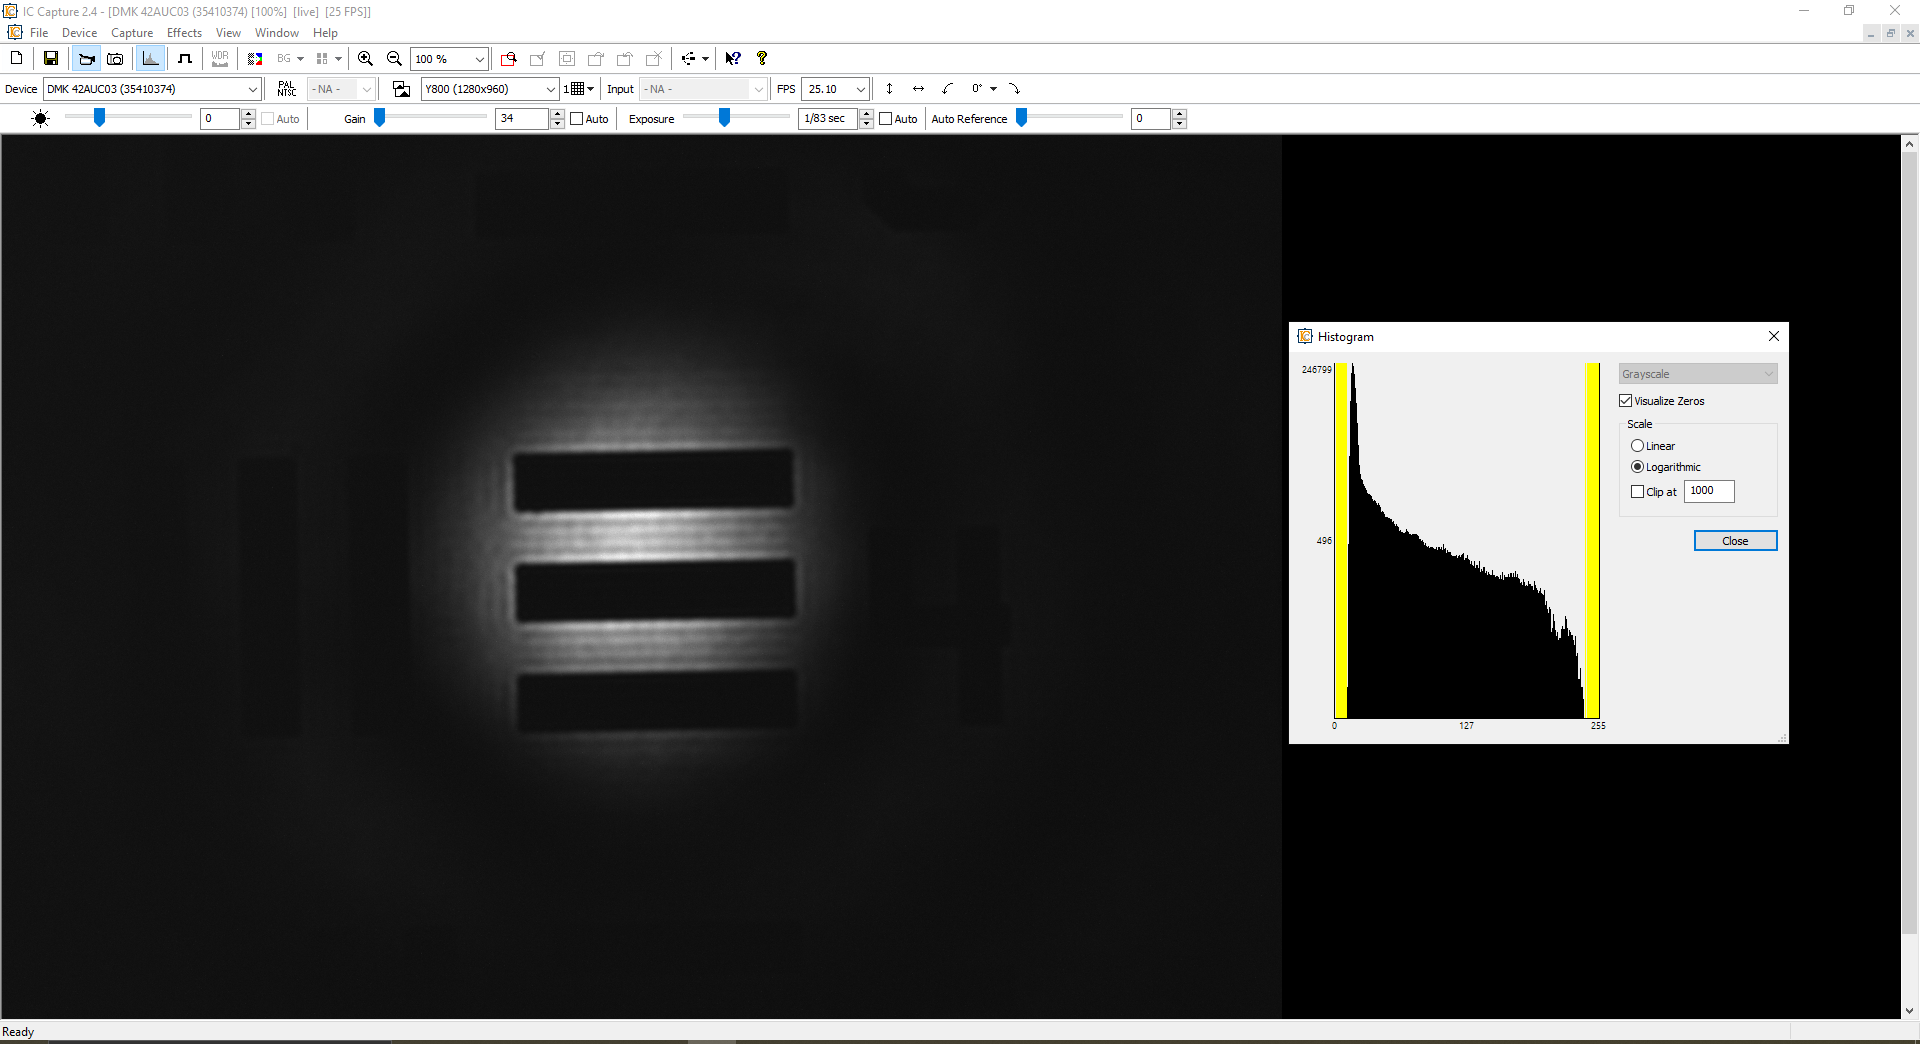
\includegraphics[width=0.45\linewidth]{nudes/AbbeTheorie/Aufgabe 2/horizontal/7te ohne.PNG}
    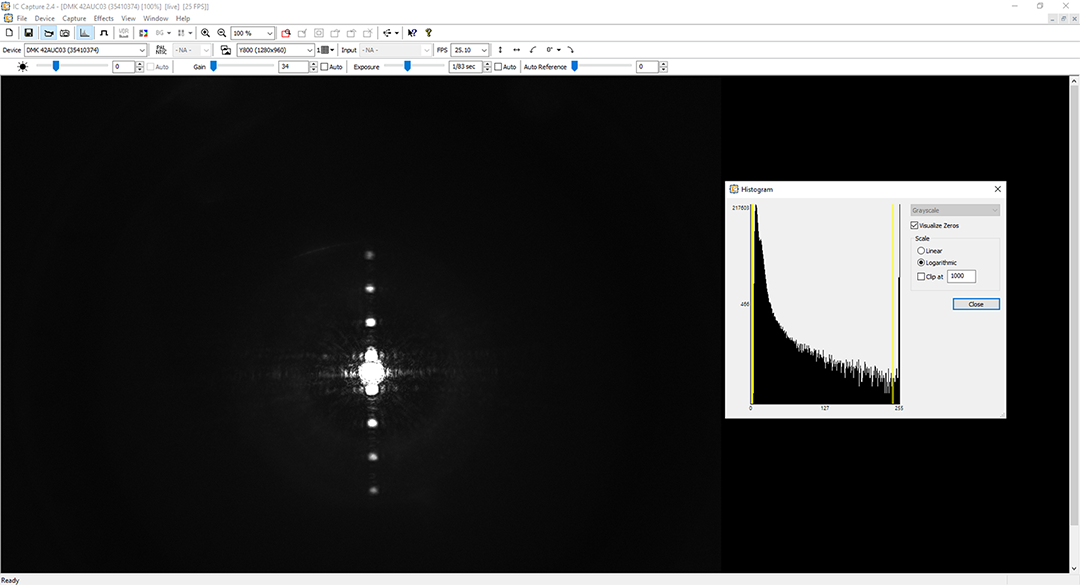
\includegraphics[width=0.45\linewidth]{nudes/AbbeTheorie/Aufgabe 2/horizontal/7te mit.PNG}
    \caption{Testobjekt mit 7 dazugehörigen Beugungsordnungen}
    \label{fig:Aufabe2-7O}
\end{figure}

\begin{figure}[H]
    \centering
    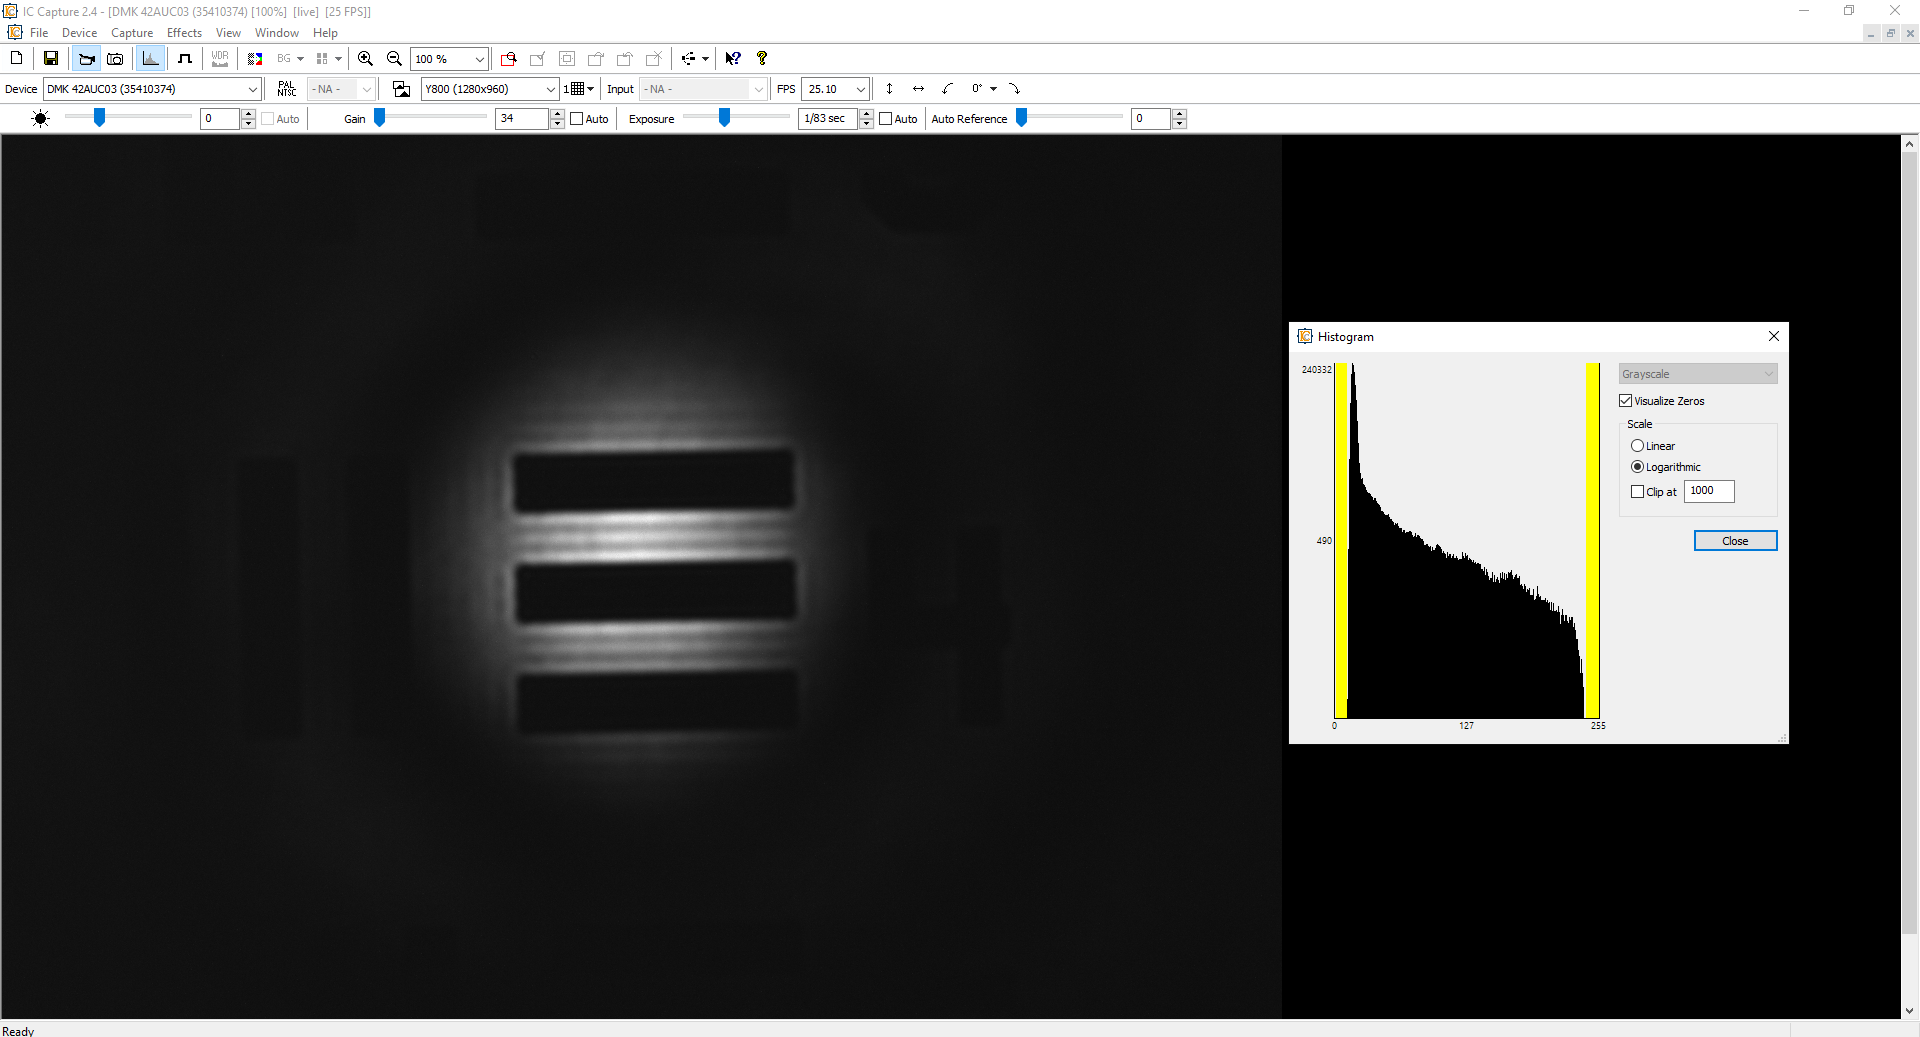
\includegraphics[width=0.45\linewidth]{nudes/AbbeTheorie/Aufgabe 2/horizontal/5te ohne.PNG}
    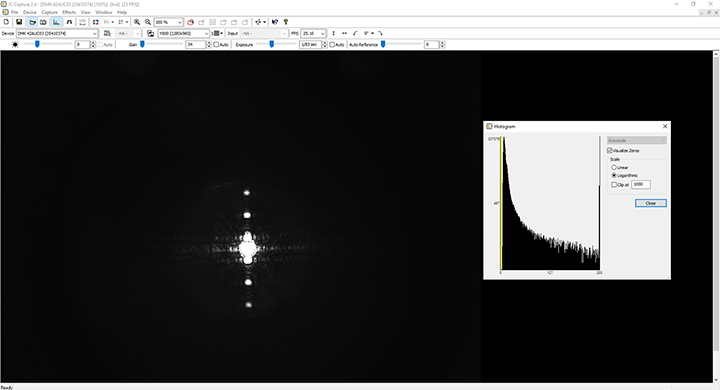
\includegraphics[width=0.45\linewidth]{nudes/AbbeTheorie/Aufgabe 2/horizontal/5te mit.PNG}
    \caption{Testobjekt mit 5 dazugehörigen Beugungsordnungen}
    \label{fig:Aufabe2-5O}
\end{figure}

\begin{figure}[H]
    \centering
    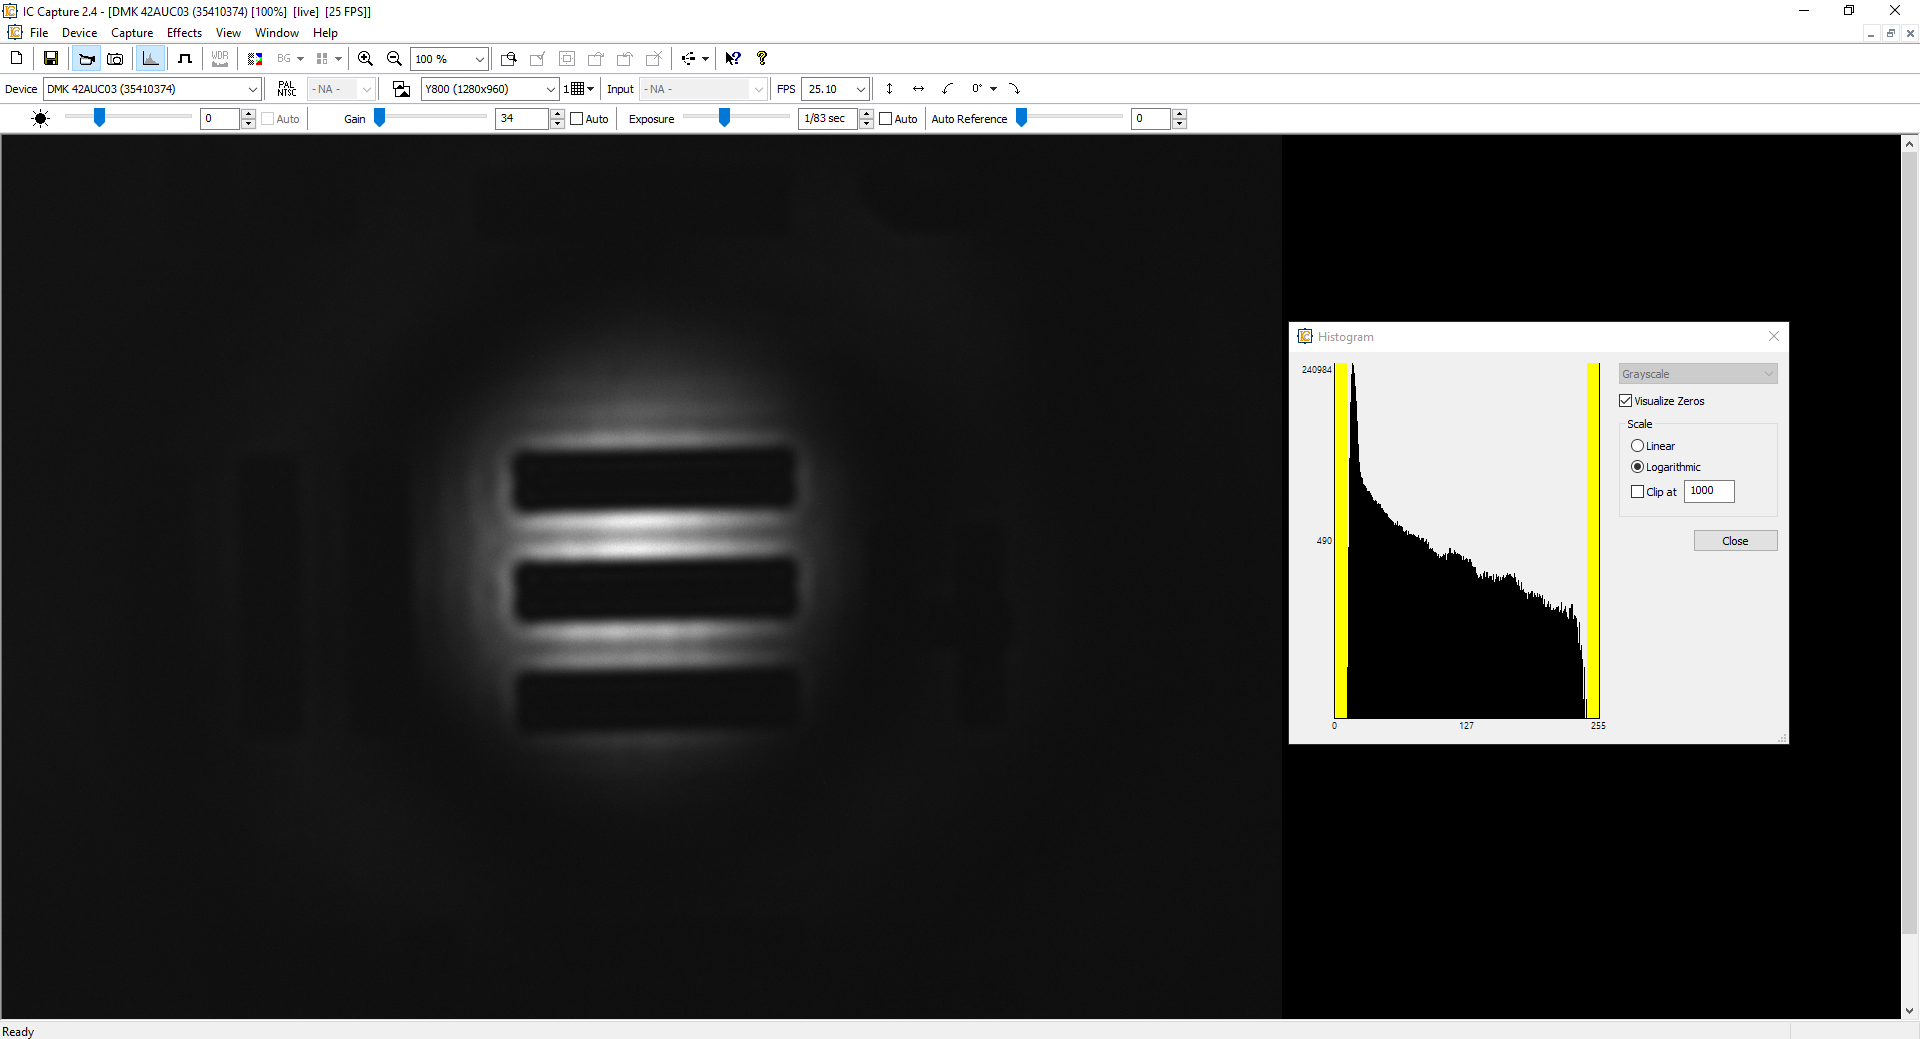
\includegraphics[width=0.45\linewidth]{nudes/AbbeTheorie/Aufgabe 2/horizontal/3te ohne.PNG}
    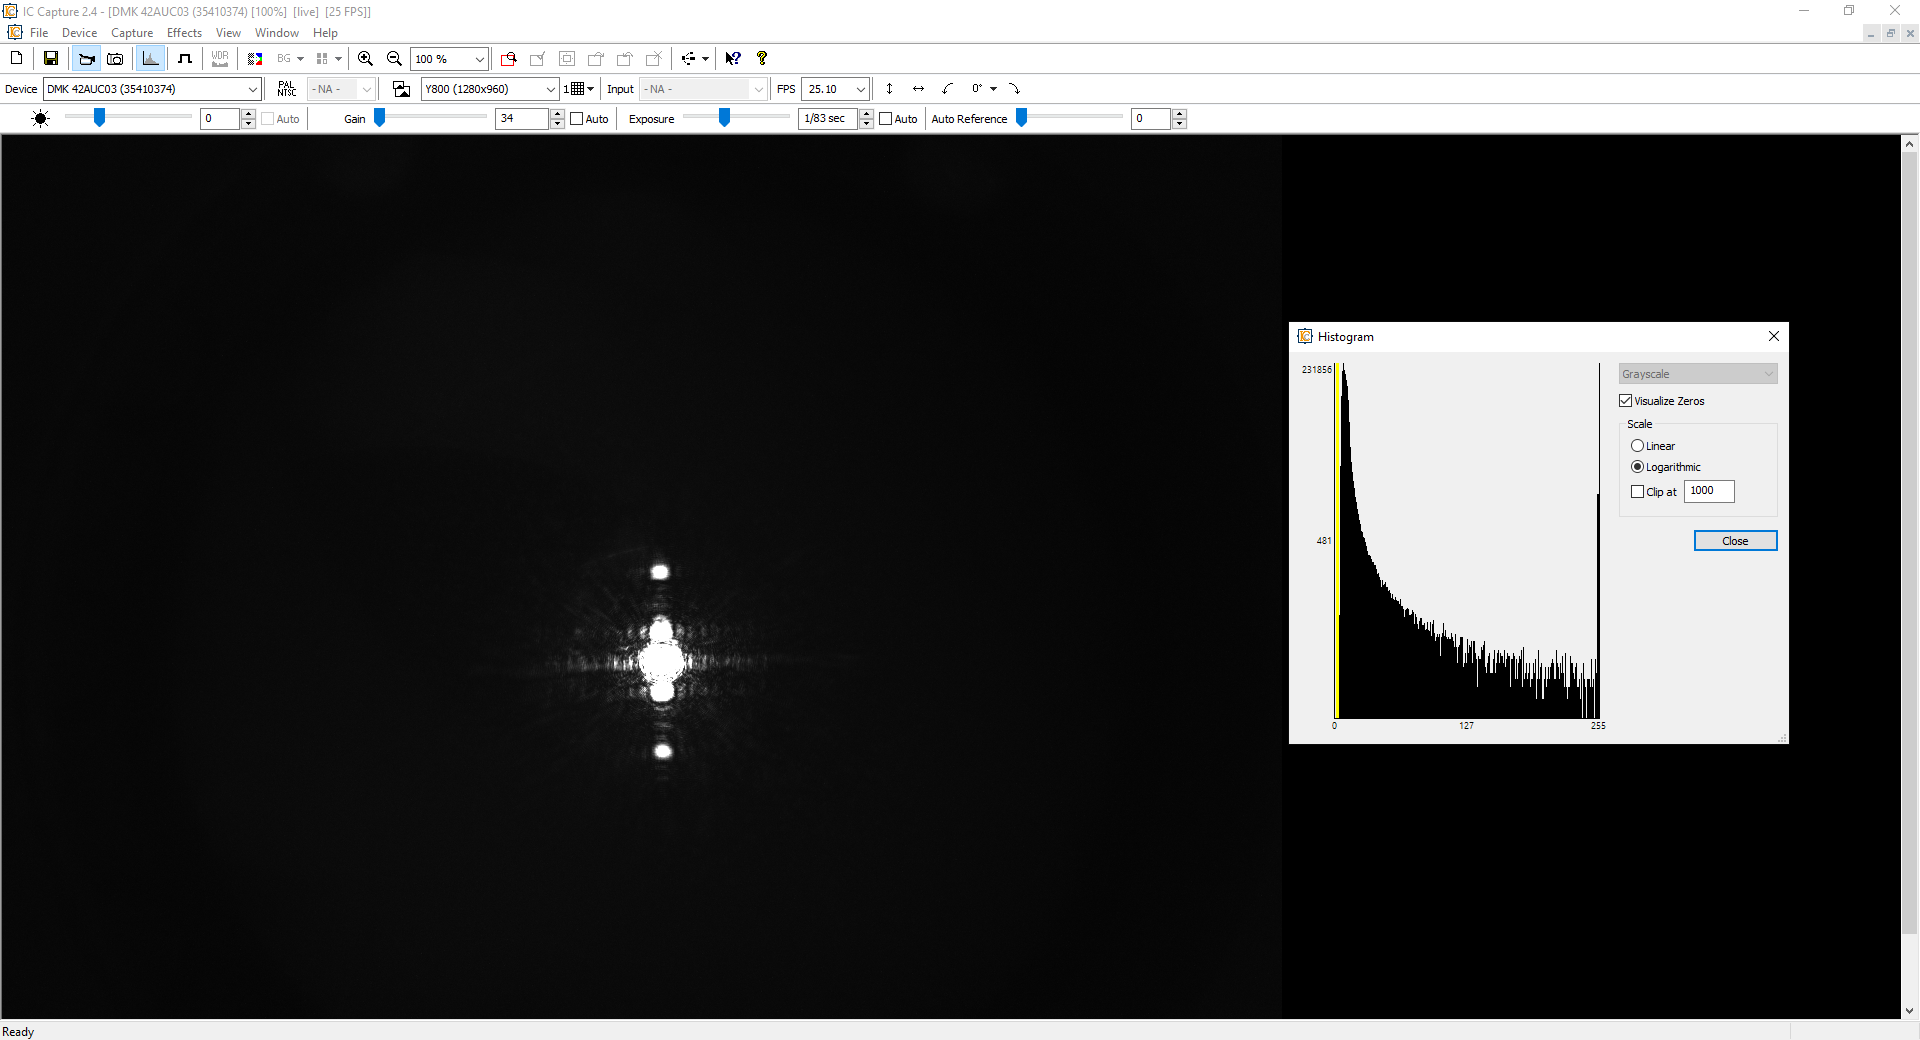
\includegraphics[width=0.45\linewidth]{nudes/AbbeTheorie/Aufgabe 2/horizontal/3te mit.PNG}
    \caption{Testobjekt mit 3 dazugehörigen Beugungsordnungen}
    \label{fig:Aufabe2-3O}
\end{figure}

\begin{figure}[H]
    \centering
    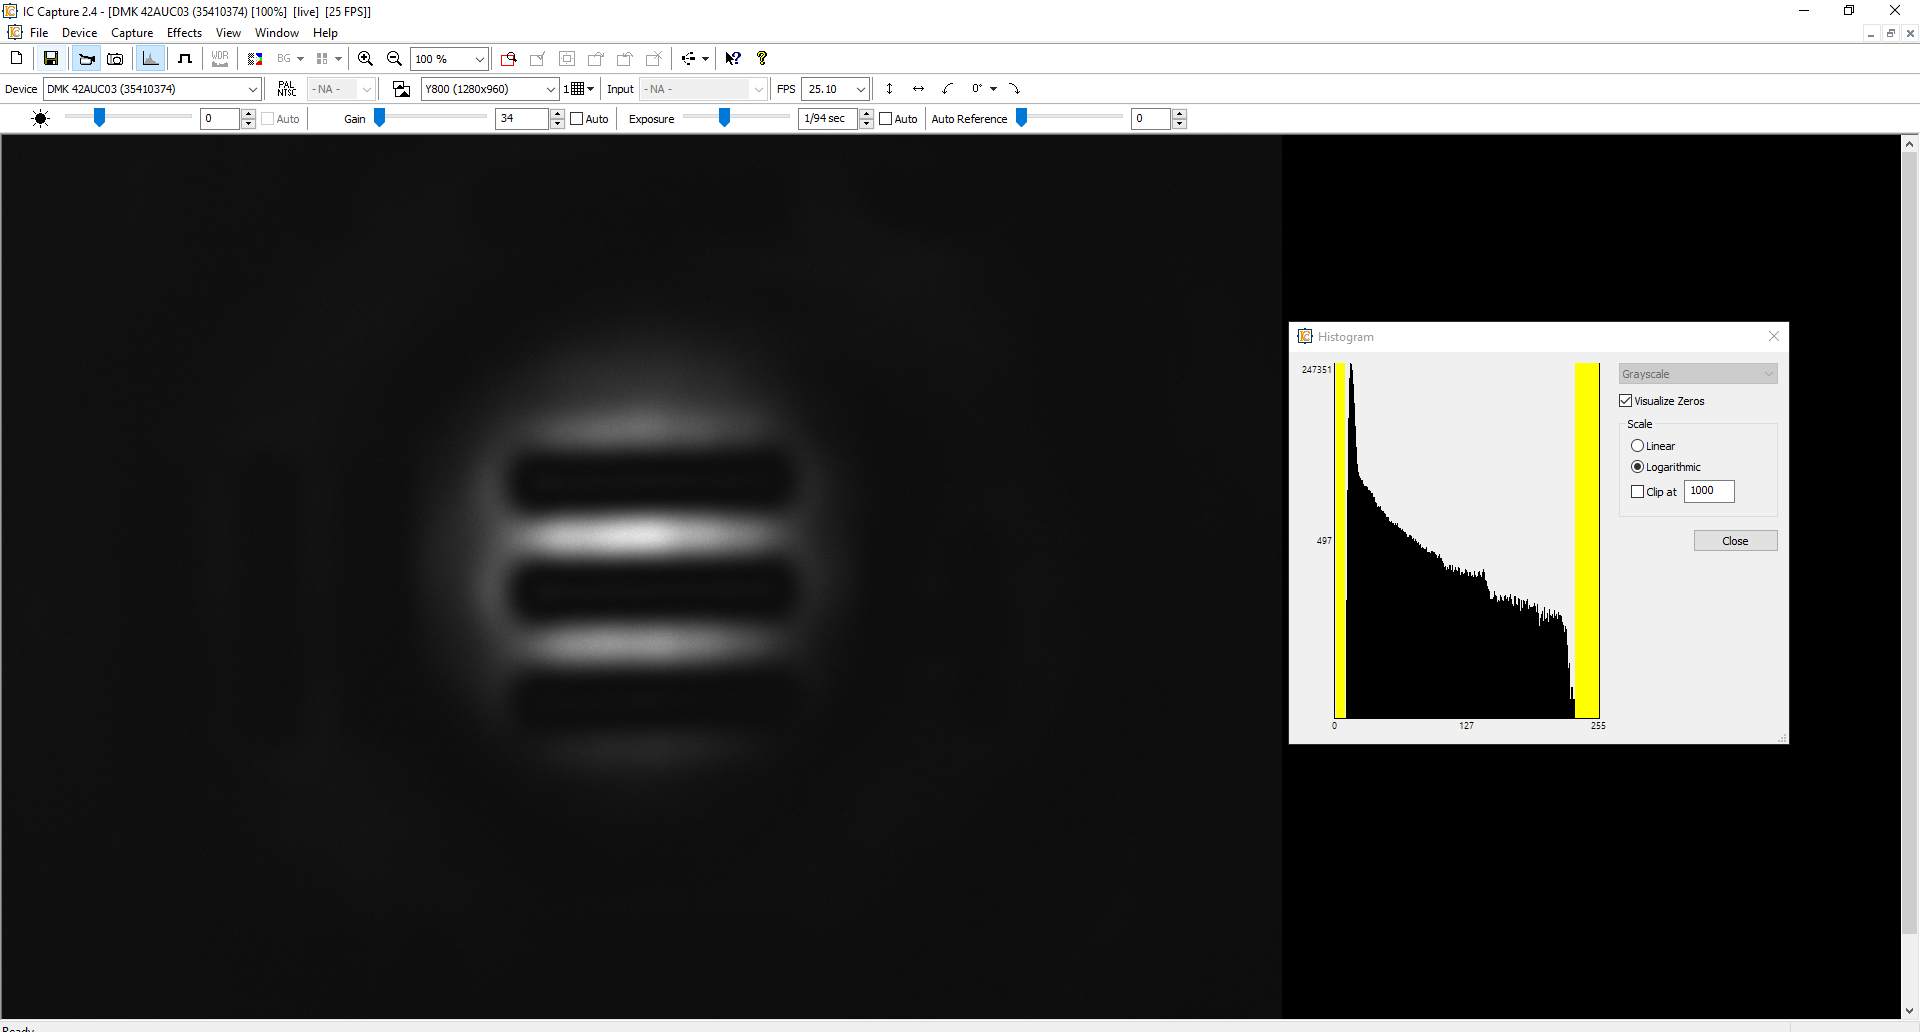
\includegraphics[width=0.45\linewidth]{nudes/AbbeTheorie/Aufgabe 2/horizontal/1te ohne.PNG}
    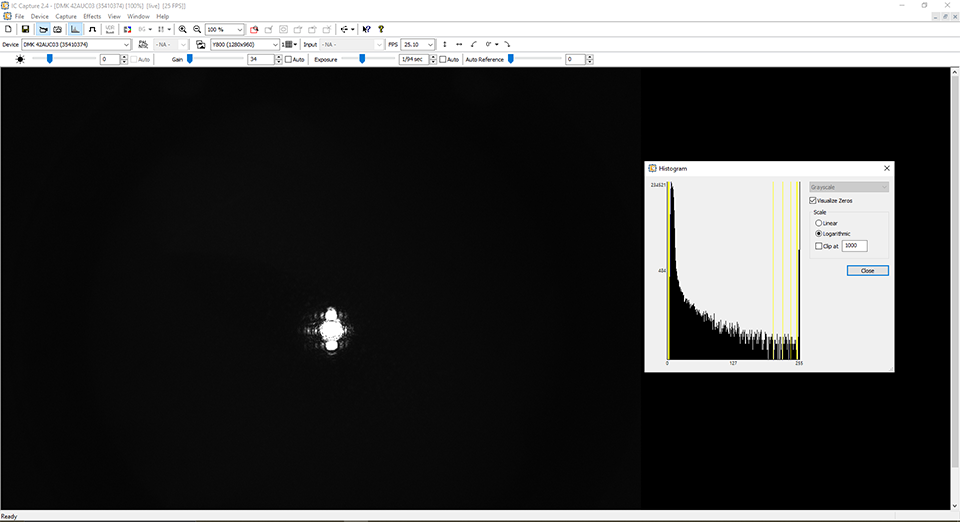
\includegraphics[width=0.45\linewidth]{nudes/AbbeTheorie/Aufgabe 2/horizontal/1te mit.PNG}
    \caption{Testobjekt mit 1 dazugehörigen Beugungsordnungen}
    \label{fig:Aufabe2-1O}
\end{figure}

\begin{figure}[H]
    \centering
    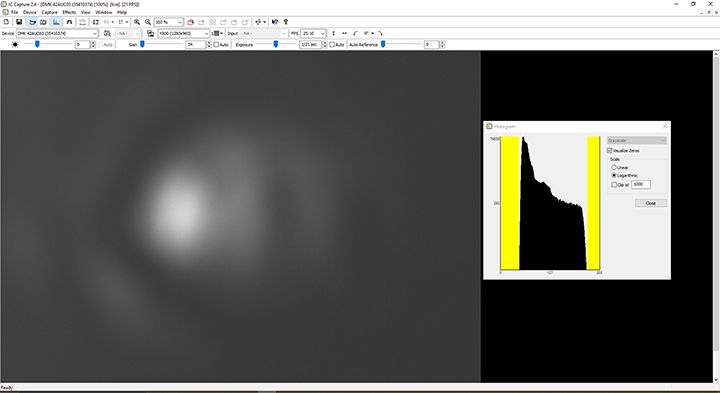
\includegraphics[width=0.45\linewidth]{nudes/AbbeTheorie/Aufgabe 2/horizontal/0te ohne.PNG}
    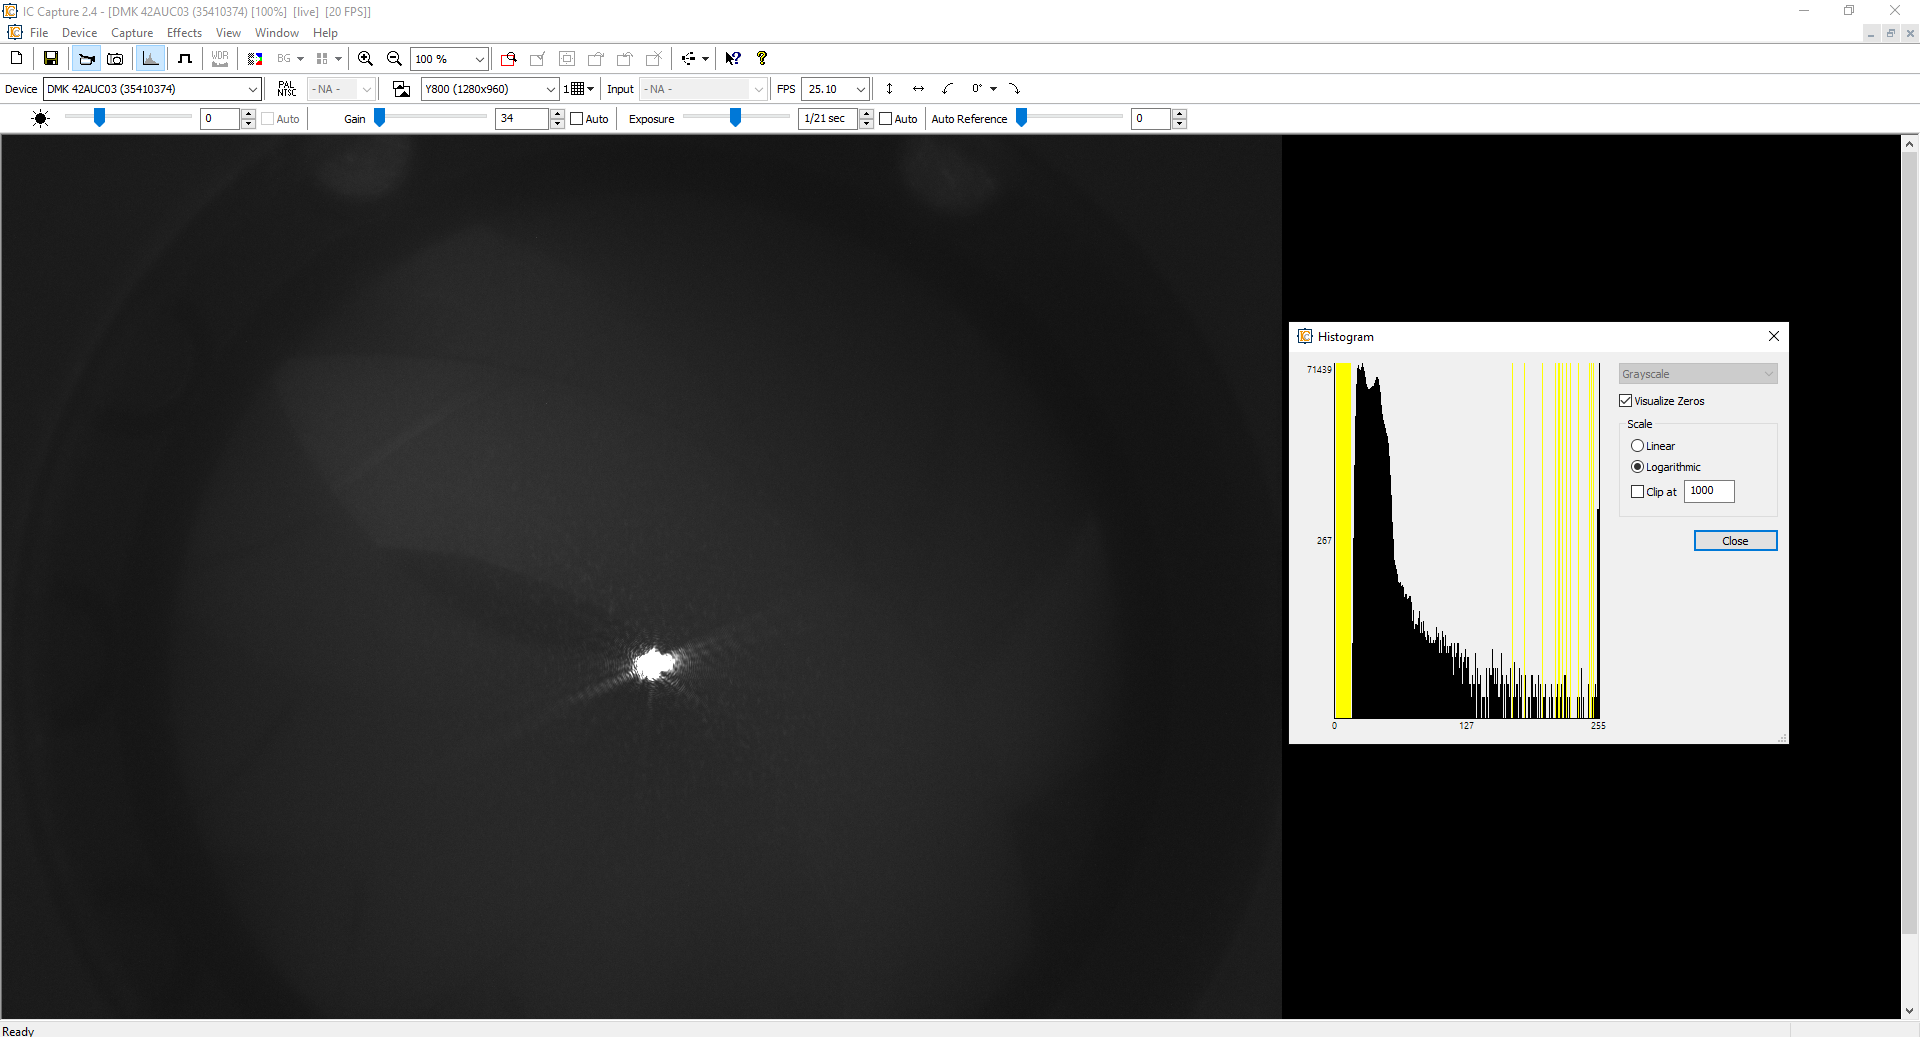
\includegraphics[width=0.45\linewidth]{nudes/AbbeTheorie/Aufgabe 2/horizontal/0te mit.PNG}
    \caption{Testobjekt mit 0 dazugehörigen Beugungsordnungen}
    \label{fig:Aufabe2-0O}
\end{figure}

\noindent
Bei der 0. und 1. Ordnung lässt sich eine Sättigung des Beugungsbildes nicht wirklich vermeiden, jedoch wurde die Belichtungszeit für ein bestmögliches Ergebniss angepasst.


\subsection{Freies Experimentieren}

Zu guter Letzt sind der Kreativität keine Grenzen gesetzt. Jedoch gibt es auch beim freien Experimentieren eine kleine Aufgabenstellung. \newline

\noindent
Zunächst sollte sich das Beugungsbild für die vertikal Objektbalken angesehen werden:

\begin{figure}[H]
    \centering
    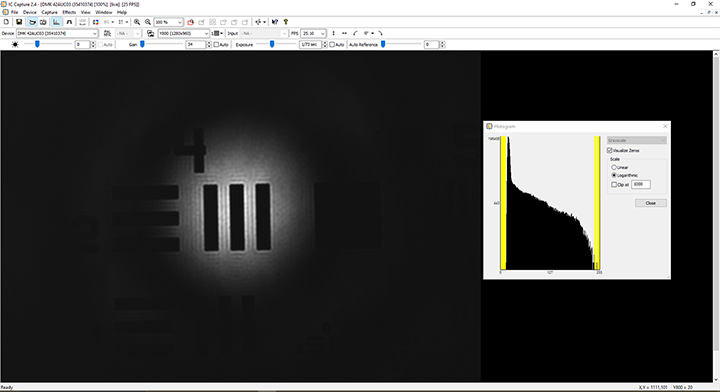
\includegraphics[width=0.45\linewidth]{nudes/AbbeTheorie/Aufgabe 3/4-2 vertikal ohne.PNG}
    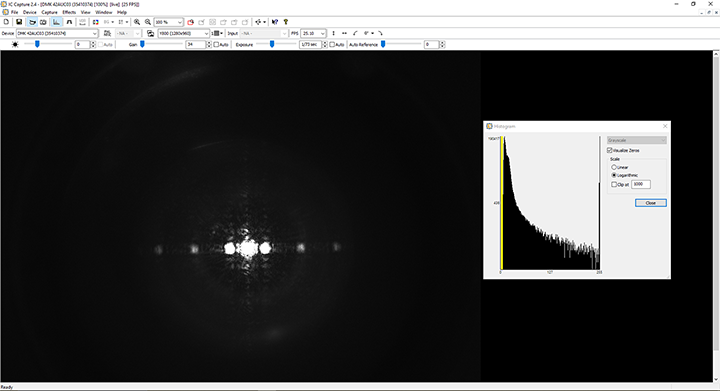
\includegraphics[width=0.45\linewidth]{nudes/AbbeTheorie/Aufgabe 3/4-2 vertikal mit.PNG}
    \caption{Testobjekt vertikal 3 Beugungsordnungen}
    \label{fig:Aufabe3-horizontal}
\end{figure}

\noindent
Weiters soll nun die nullte Ordnung mit der Drahtblende des Filterrads B ausgeblendet und das Ergebniss visuell dargestellt werden.

\begin{figure}[H]
    \centering
    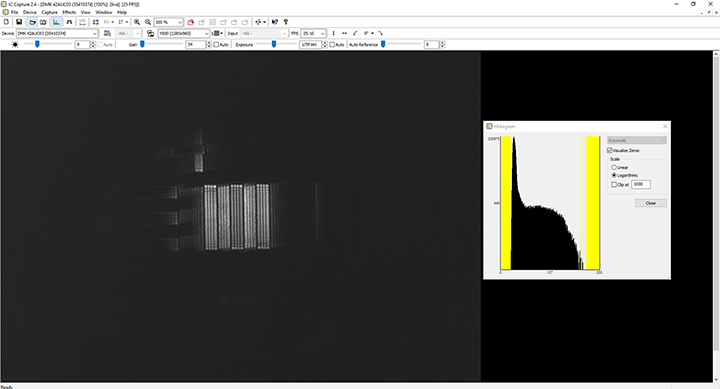
\includegraphics[width=0.45\linewidth]{nudes/AbbeTheorie/Aufgabe 3/4-2 ohne 0te ohne.PNG}
    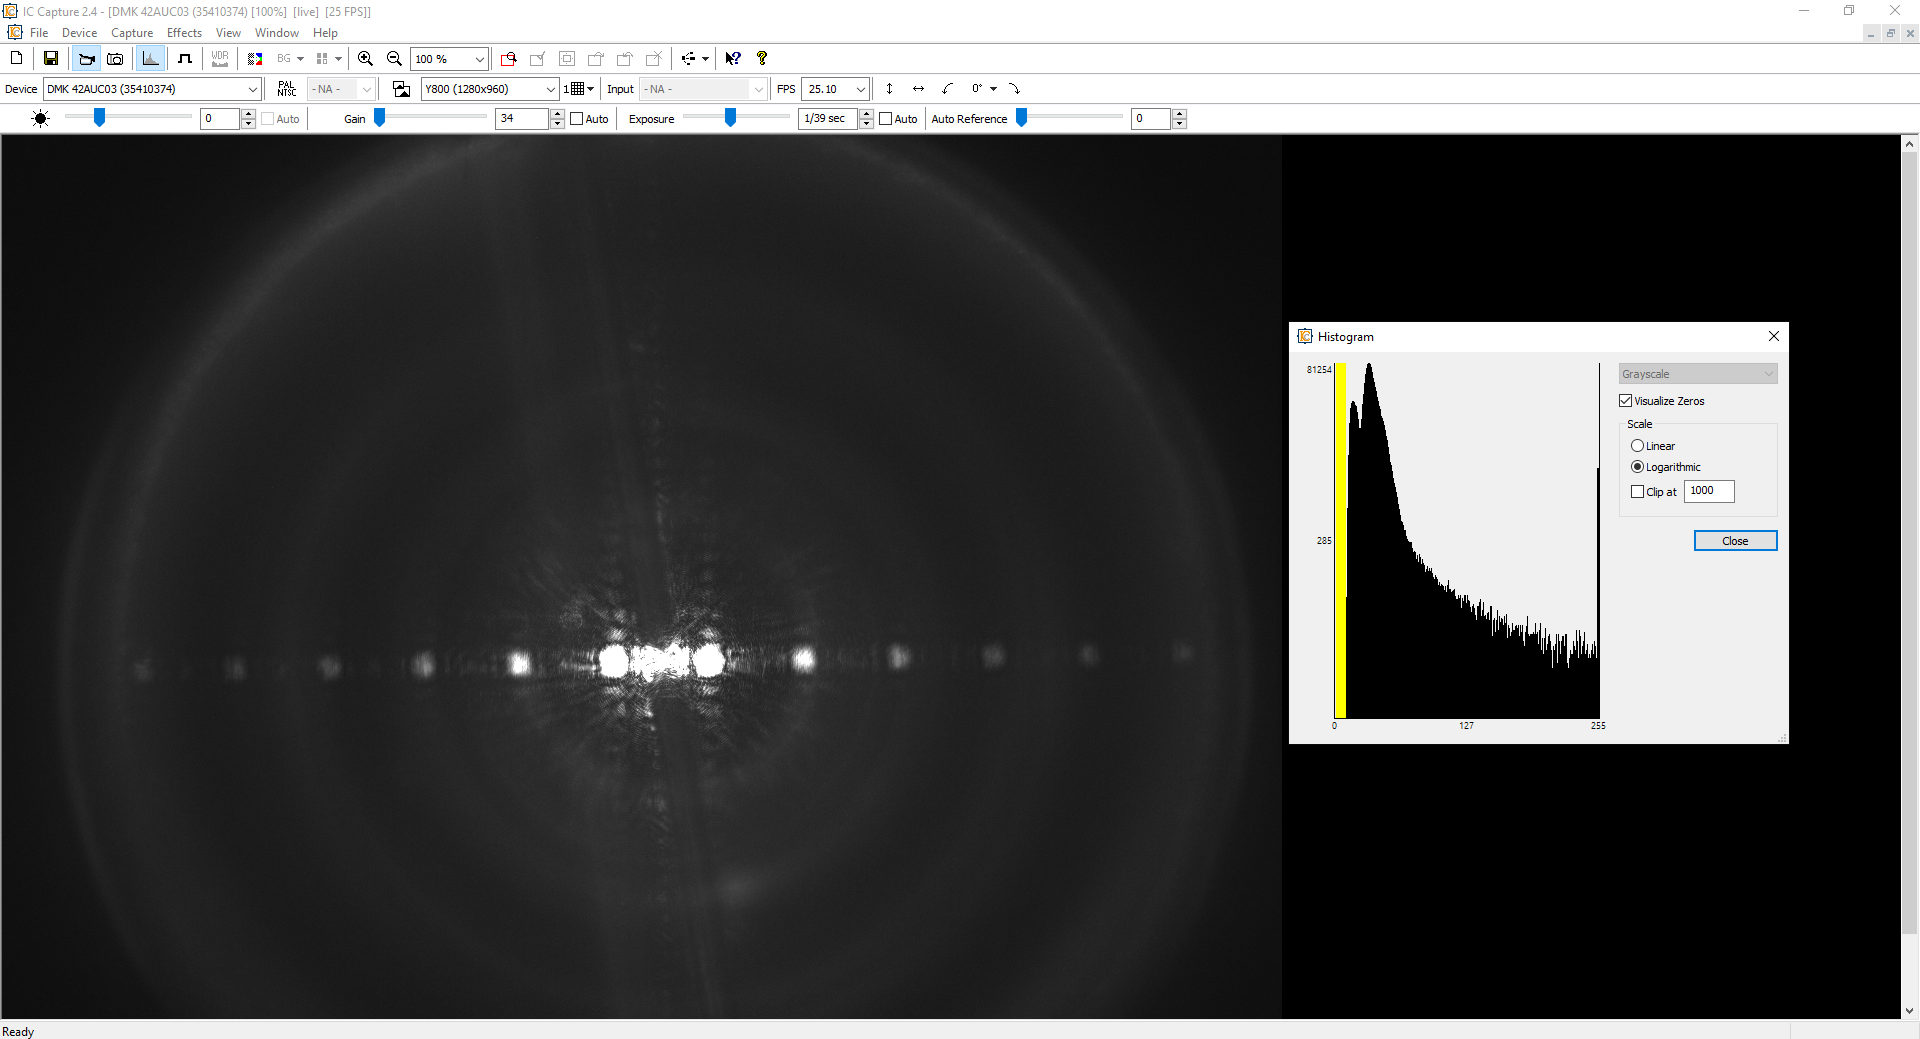
\includegraphics[width=0.45\linewidth]{nudes/AbbeTheorie/Aufgabe 3/4-2 ohne 0te mit.PNG}
    \caption{Testobjekt und Beugungsordnungen ohne Ordnung 0}
    \label{fig:Aufabe3-ohneNullte}
\end{figure}



\section{Auswertung und Unsicherheitsanalyse} %Nicht nur zahlen angeben ------------------------------

In der Auswertung werden zur erhöhten Genauigkeit durchgehend ungerundete Werte bis zu den Endergebnissen verwendet und nur zur Darstellung gerundet. \\
Zur Berechnung der Unsicherheiten wird, wenn nicht anders angegeben, die Größtunsicherheitsmethode verwendet.


\subsection{Quantitative Bestimmung des Auflösungsvermögens}

Um das Auflösungsvermögen zu bestimmen, werden zunächst die gewonnen Daten aus den Tabellen \ref{tab:MessungenAuflösungsvermögenRot} und \ref{tab:MessungenAuflösungsvermögenBlau} mit Hilfe der Tabelle \ref{tab:fR-Tabelle} für die räumlichen Frequenzen ausgewertet.
Die Unsicherheit setzt sich dabei aus der Mittelwertsformel \ref{eq:avg} der Abweichung zwischen dem Wert der räumlichen Frequenz und der Unsicherheitselemente zusammen.

\begin{table}[H]
    \centering
    \caption{Umrechnen in die räumliche Frequenz für rotes Licht}
    \label{tab:MessungenRäumliche FrequenzRot}
    \resizebox{\columnwidth}{!}{\begin{tabular}{|l|l|l|l|l|l|}
        \hline
        Nr. & Blende / mm & Räumliche Frequenz / $\frac{1}{mm}$ & \multicolumn{2}{|c|}{Unsicherheitselemente / $\frac{1}{mm}$} & Unsicherheit $\Delta f_{R}$ / $\frac{1}{mm}$ \\
        \hline
        1 & 2 &  45.3 & 40.3 &  50.8 &  5.25 \\
        2 & 3 &  64.0 & 57.0 &  71.8 &  7.40 \\
        3 & 6 & 102.0 & 90.5 & 114.0 & 11.75 \\
        \hline
    \end{tabular}}
\end{table}

\begin{table}[H]
    \centering
    \caption{Umrechnen in die räumliche Frequenz für blaues Licht}
    \label{tab:MessungenRäumlicheFrequenzBlau}
    \resizebox{\columnwidth}{!}{\begin{tabular}{|l|l|l|l|l|l|}
        \hline
        Nr. & Blende / mm & Räumliche Frequenz / $\frac{1}{mm}$ & \multicolumn{2}{|c|}{Unsicherheitselement / $\frac{1}{mm}$} & Unsicherheit $\Delta f_{R}$ / $\frac{1}{mm}$ \\
        \hline
        1 & 2 &  50.8 &  45.3 & 57.0 &   5.85 \\
        2 & 3 &  80.6 &  71.8 & 90.5 &   9.35 \\
        3 & 6 & 128.0 & 114.0 & 144.0 & 15.00 \\
        \hline
    \end{tabular}}
\end{table}

\noindent
Weiters wird dann mittels Formel \ref{eq:WZ-dExp} das Auflösungsvermögen und mittels Formel \ref{eq:WZ-NA} die numerische Apertur berechnet.

\begin{table}[H]
    \centering
    \caption{Berechnete numerische Apertur}
    \label{tab:BerechneteNA}
    \begin{tabular}{| l | l | l |}
        \hline
        Nr. & Blende / mm & NA / 1\\
        \hline
        1 & 2 & 0.0167 $\pm$ 0.0003 \\
        2 & 3 & 0.0250 $\pm$ 0.0005 \\
        3 & 6 & 0.0500 $\pm$ 0.0008 \\
        \hline
    \end{tabular}
\end{table}

\begin{table}[H]
    \centering
    \caption{Berechnetes Auflösungsvermögen rotes Licht}
    \label{tab:BerechneteAVrot}
    \begin{tabular}{| l | l | l | l |}
        \hline
        Nr. & Blende / mm & $d_{exp}$ / $\mu m$\\
        \hline
        1 & 2 & 0.022  $\pm$ 0.003  \\
        2 & 3 & 0.0156 $\pm$ 0.0019 \\
        3 & 6 & 0.0098 $\pm$ 0.0012 \\
        \hline
    \end{tabular}
\end{table}

\begin{table}[H]
    \centering
    \caption{Berechnetes Auflösungsvermögen blaues Licht}
    \label{tab:BerechneteAVblau}
    \begin{tabular}{| l | l | l |}
        \hline
        Nr. & Blende / mm & $d_{exp}$ / $\mu m$\\
        \hline
        1 & 2 & 0.020  $\pm$ 0.003  \\
        2 & 3 & 0.0124 $\pm$ 0.0019 \\
        3 & 6 & 0.0078 $\pm$ 0.0012 \\
        \hline
    \end{tabular}
\end{table}

\noindent
Nachdem diese Werte festgehalten sind, kann nun mittels Formel \ref{eq:WZ-dTheo}, eingebunden in qti-Plot, der theoretische Verlauf des Auflösungsvermögens dargestellt und mit den experimentell resultierten Werten vergleichen.
Als Unsicherheit für die Wellenlänge $ \lambda $ wurden für rotes und blaues Licht $\pm$ 10 $\mu m$ eingesetzt.

\begin{figure}[H]
    \centering
    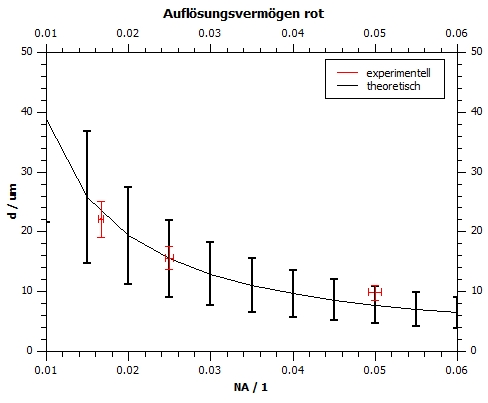
\includegraphics[width=0.6\linewidth]{nudes/AuflösungsvermögenPlotRot.jpg}
    \caption{Theoretisches und experimentelles Auflösungsvermögen auf NA rotes Licht}
    \label{fig:AuflösungsvermögenPlotRot}
\end{figure}

\begin{figure}[H]
    \centering
    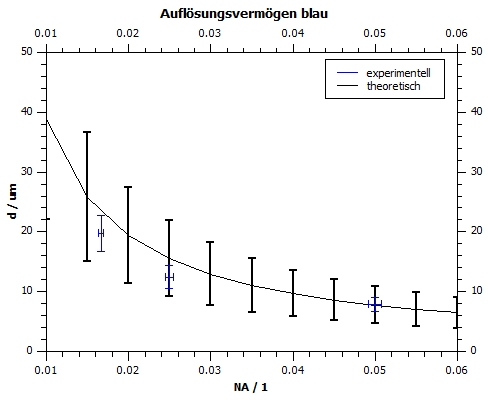
\includegraphics[width=0.6\linewidth]{nudes/AuflösungsvermögenPlotBlau.jpg}
    \caption{Theoretisches und experimentelles Auflösungsvermögen auf NA blaues Licht}
    \label{fig:AuflösungsvermögenPlotBlau}
\end{figure}


\subsection{Zusammenhang Auflösung Spaltgitterbildes und Anzahl Beugungsordnungen}

Der Zusammenhang zwischen Auflösungsvermögen und der Anzahl der Beugungsordnungen lässt sich in Abbildungen \ref{fig:Aufabe2-7O} - \ref{fig:Aufabe2-0O} eindeutig erkennen.
Eine genügende verkleinerung des Blendendurchmessers bewirkt eine reduzierung der Beugungsordnung, was mit Hilfe der Hilfslinse L3 in den eben genannten Abbildungen visualisiert werden konnte.


\subsection{Freies experimentieren}

Beim freien experimentieren sollte nun eine Verbindung zur Fourieroptik gezeigt werden.
Dafür wurden die Bilder \ref{fig:Aufabe2-7O} bis \ref{fig:Aufabe2-3O} mittels Software ImageJ näher unter die Lupe genommen.
Die Intensität der hellen Bereiche zwischen zwei Balken eines Elementes wurden geplotet, was in den foldenden Abbildungen zu sehen ist.

\begin{figure}[H]
    \centering
    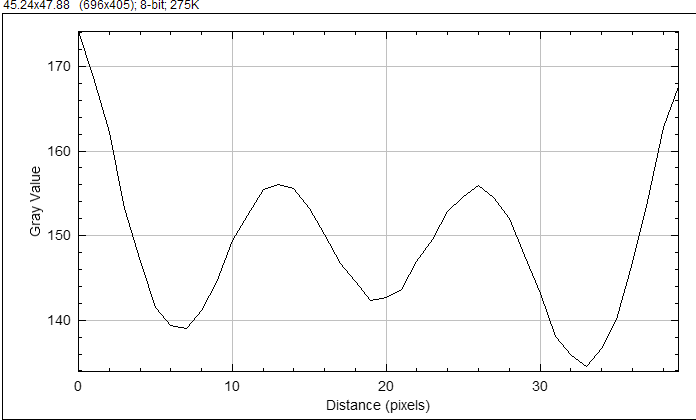
\includegraphics[width=0.6\linewidth]{nudes/A3_O7_Plot.png}
    \caption{Intensitätsplot des 7. Ordnungsbildes}
    \label{fig:IntensitätsPlotO7}
\end{figure}

\begin{figure}[H]
    \centering
    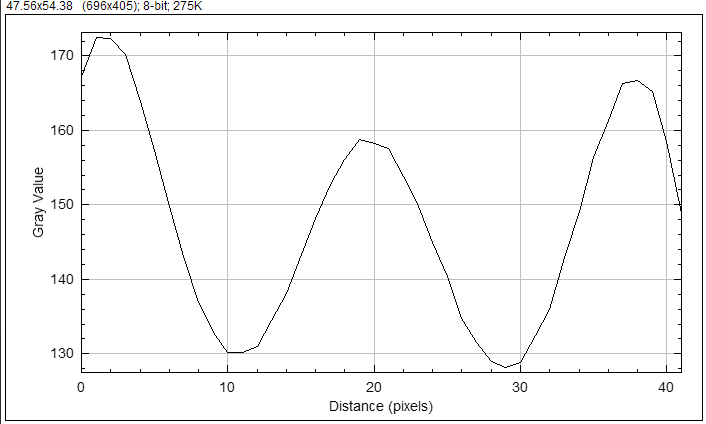
\includegraphics[width=0.6\linewidth]{nudes/A3_O5_Plot.png}
    \caption{Intensitätsplot des 5. Ordnungsbildes}
    \label{fig:IntensitätsPlotO5}
\end{figure}

\begin{figure}[H]
    \centering
    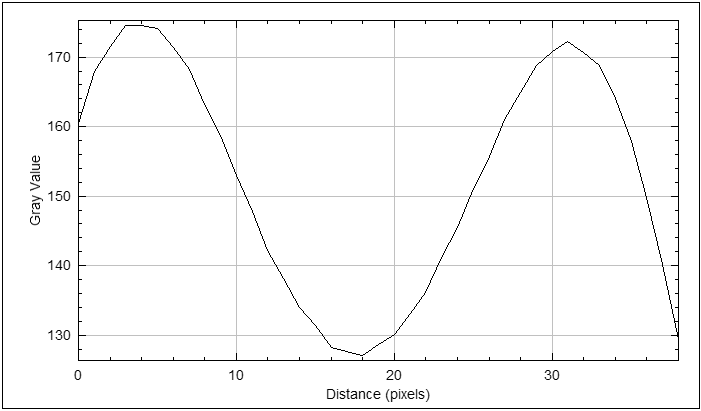
\includegraphics[width=0.6\linewidth]{nudes/A3_O3_Plot.png}
    \caption{Intensitätsplot des 3. Ordnungsbildes}
    \label{fig:IntensitätsPlotO3}
\end{figure}

\noindent
Mittels Fouriertransformation der Beugungsverteilung ist das Bild eines Objektes gegeben. Sobald räumliche Strukturen in der Beugungsverteilung fehlen, gibt es dort keine Fouriergrößen im Bild (Verwaschene Konturen). 
Dies ist darauf zurückzuführen, dass diese Strukturen durch die Blende abgeschnitten werden. 
Schließt man also die Blende, sollte der Breich zwischen zwei Blöcken eines Elementes immer verwaschener werden, was sich gut in den Abbildungen \ref{fig:Aufabe2-7O} - \ref{fig:Aufabe2-0O} erkennen lässt.
Auch die Intensitätsplots weißen in diesen Bereichen weniger Schwankungen auf. \cite{dem2}



\section{Diskussion} %diskussion der Unsicherheiten und Ergebnisse und evtl. verlgeich mit Literatur ------------------------------

\subsection{Vertrautmachen mit dem Versuch}

Da durch das schließen der Blende die numerische Apertur laut Formel \ref{eq:WZ-NA} größer wird, wird das Auflösungsvermögen laut Formel \ref{eq:Auflösungsvermögen} kleiner. Somit werden Elemente, die vorher noch gut erkennbar waren, plötzlich unscharf.


\subsection{Quantitative Bestimmung des Auflösungsvermögens}

Die experimentell ermittelten Werte überlagern sich laut Abbildungen \ref{fig:AuflösungsvermögenPlotRot} und \ref{fig:AuflösungsvermögenPlotBlau} mit dem theoretischen Verlauf des Auflösungsvermögens, was für eine richtige Versuchsdurchführung und Auswertung spricht.


\subsection{Zusammenhang Auflösung Spaltgitterbildes und Anzahl Beugungsordnungen}

Die Beugungsordnung verändert sich wie zu erwarten mit dem Linsenöffnungsdurchmesser, was in den ermittelten Abbildungen \ref{fig:Aufabe2-7O} - \ref{fig:Aufabe2-0O} deutlich zu sehen ist.


\subsection{Freies Experimentieren}

Betrachtet man das Ordnungsbild der vertikalen Balken, so lässt sich erkennen, dass die Ordnungen nun um 90° gedreht sind und nun eine horizontale Linie bilden. \newline

\noindent
Mit einer Abstandserhöhung der Balken der Elemente verändern sich die Zahl und Positionen der Intensitätsmaxima. \newline

\noindent
In den Abbildungen \ref{fig:Aufabe2-7O} - \ref{fig:Aufabe2-0O} lassen sich außerdem Beugungserscheinungen normal zu den Maxima erkennen. 
Ein Grund dafür könnten Interferenzen verschieden gebeugter Lichtwellen sein, die so gebeugt werden, dass sie ein horizontales Erscheinungsbild erzeugen.

\noindent
Wird die nullte Ordnung abgedeckt, so verschwimmt das Testelementbild und es lassen sich keine schönen Balken mehr erkennen.
Außerdem ist nicht zu übersehen, dass die Farben nun invertiert, also schwarz wird zu weiß und umgekehrt, sind.
Dies lässt sich auf das Prinzip der Dunkelfeldmikroskopie zurückführen, bei der die Lichtstrahlen, die normalerweiße durch eine Probe gehen, blockiert werden und nur schräg einfallende Strahlen den Sensor erreichen. \cite{dunkelfeldmikroskopie}



\section{Zusammenfassung} %klare, übersichtliche vollständige beantwortung der Aufgabenstellung ------------------------------

\subsection{Quantitative Bestimmung des Auflösungsvermögens}

\begin{table}[H]
    \centering
    \caption{Berechnete numerische Apertur}
    \label{tab:BerechneteNA}
    \begin{tabular}{| l | l | l | l |}
        \hline
        Nr. & Blende / mm & NA / 1 & $\Delta NA$ / 1 \\
        \hline
        1 & 2 & 0.0167 & 0.0003 \\
        2 & 3 & 0.0250 & 0.0005 \\
        3 & 6 & 0.0500 & 0.0008 \\
        \hline
    \end{tabular}
\end{table}

\begin{table}[H]
    \centering
    \caption{Berechnetes Auflösungsvermögen rotes Licht}
    \label{tab:BerechneteAVrot}
    \begin{tabular}{| l | l | l | l |}
        \hline
        Nr. & Blende / mm & $d_{exp}$ / $\mu m$ & $\Delta d_{exp}$ / $\mu m$ \\
        \hline
        1 & 2 & 0.022  & 0.003  \\
        2 & 3 & 0.0156 & 0.0019 \\
        3 & 6 & 0.0098 & 0.0012 \\
        \hline
    \end{tabular}
\end{table}

\begin{table}[H]
    \centering
    \caption{Berechnetes Auflösungsvermögen blaues Licht}
    \label{tab:BerechneteAVblau}
    \begin{tabular}{| l | l | l | l |}
        \hline
        Nr. & Blende / mm & $d_{exp}$ / $\mu m$ & $\Delta d_{exp}$ / $\mu m$ \\
        \hline
        1 & 2 & 0.020  & 0.003  \\
        2 & 3 & 0.0124 & 0.0019 \\
        3 & 6 & 0.0078 & 0.0012 \\
        \hline
    \end{tabular}
\end{table}


\subsection{Zusammenhang Auflösung Spaltgitterbildes und Anzahl Beugungsordnungen}

Der Zusammenhang zwischen Auflösungsvermögen und der Anzahl der Beugungsordnungen lässt sich in Abbildungen \ref{fig:Aufabe2-7O} - \ref{fig:Aufabe2-0O} eindeutig erkennen.



\newpage
\section{Anhang}

In diesem Abteil werden die Unsicherheitsrechnungen zur eventuellen Fehlersuche abgebildet. Für Unsicherheiten von Größeren Tabellen wird jeweils die Rechnung des ersten Wertes als Beispiel für die restlichen Größen gezeigt.

\begin{figure}[H]
    \centering
    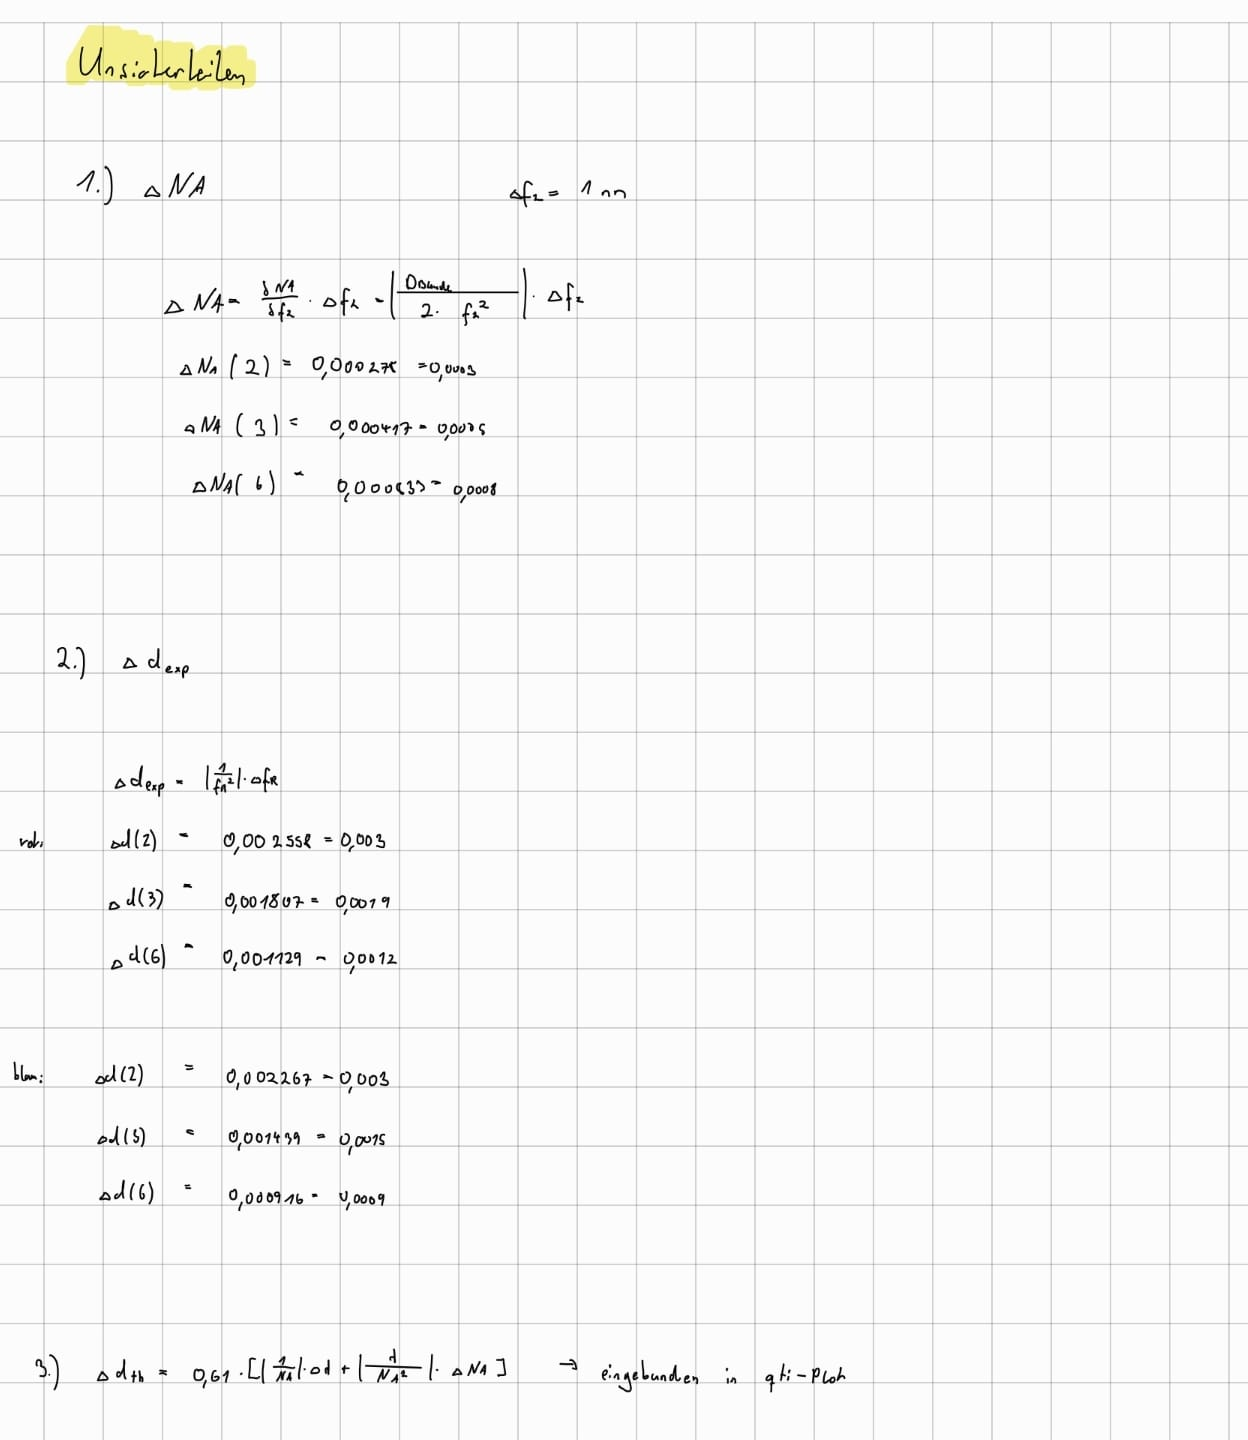
\includegraphics[width=0.8\linewidth, angle=0]{nudes/Unsicherheiten1.jpg}
    \caption{Unsicherheitsrechnungen}
    \label{fig:Unsicherheitsrechnungen1}
\end{figure}

\printbibliography[heading=bibintoc]
\end{document}
